
\documentclass[12pt,journal,letterpaper,oneside,onecolumn]{IEEEtran}
%\addtolength{\voffset}{0.1in}
%\addtolength{\hoffset}{0.1in}
\usepackage[pdftex]{graphicx}

% correct bad hyphenation here if needed
\hyphenation{op-tical net-works semi-conduc-tor}


\begin{document}
%
\title{Unsupervised generation of tradeable topic indices from Financial reports through Latent Dirichlet Analysis}

\author{
Marcel Lee
and Alan Spark% <-this % stops a space
%\thanks{Author A's affiliation}% <-this % stops a space
%\thanks{Author B's affiliation}% <-this % stops a space
}


% The paper headers
%\markboth{Journal of Financial and Quantitative Analysis}
%{Author A and author B}

% make the title area
\maketitle

% As a general rule, do not put math, special symbols or citations
% in the abstract or keywords.
\begin{abstract}
The movement of publicly traded equities can be modeled as a combination of 
underlying risk factors that are not directly observable in the market. The  model in this paper combines financial statement based information, in particular the the 10-K and 10-Q reports, with price information to isolate these hidden risk factors.
It uses the dynamic variant of Blei's Latent Dirichlet Allocation model to split each stock into T topic proportions. These are then interpreted as the risk factor proportions.
Thus, at each time point stocks can be represented as a vector in T dimensional topic/risk space.
The model then uses the QR factorization algorithm with column pivoting to calculate the optimal weights that these factors need to be combined to find the standard normal basis $([1,0,0,...], [0,1,0...], [0,0,1....])$.
The standard normal basis will correspond directly to the risk factors to be extracted. The optimal weights will indicate the equity proportions necessary to combine the equities into pure risk factors.
\end{abstract}

\section{Introduction}
Prices of traded stocks are driven by a multitude of risk factors. Depending on the model these may include sector (e.g. automobile, consumers), country risk (e.g. US, France, etc), size, reputational risk, human resource risk, political risk, etc.
Every traded stock can thus be modeled as a composition of risks. Despite the thousands of sector and thematic indices released every year by fund management companies, it is currently not possible trade the risk factors in isolation. This is because the actual risk factor composition of the individual stocks is unknown. 
\begin{figure}
    \centering
	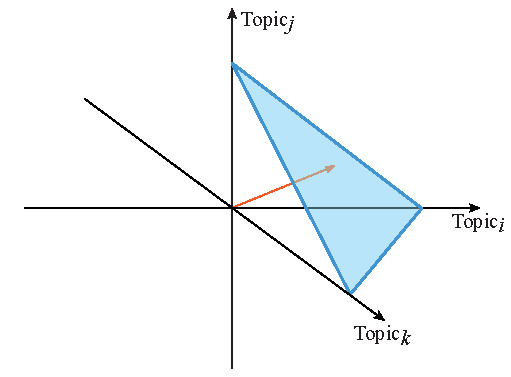
\includegraphics[width=0.5\linewidth]{images/vector_representation.pdf}	\caption{Vector representation of a stock in the Topic's space. Red vector represent $\vec{\theta}$ in 3 dimensions/topics space}
	\label{fig:companies-topics-distribution}       
\end{figure}

For example, a fund manager may have strong views on airlines or IT, but cannot trade this risk individually as every single airline or IT stock is a composition of risks which besides pure airline or IT risk also includes other risk factors. 
In financial literature the problem of contamination of a hedge through other risk factors is known \textit{basis risk}.
In linear algebra terms a basis of a space is a set of elements such that every element in the space may be expressed as a linear combination of elements in this basis.
This paper is an attempt to create such a basis of the set of risk factors through information released by the company itself, in particular the 10-K and 10-Q reports or the national equivalents of the annual and quarterly reports.

A machine learning technique called Latent Dirichlet Allocation is
used to split text documents into components called topics.
A topic in this case is a frequency distribution over words.
LDA is applied on the financial reports of the company.
The topic proportions are then interpreted as the actual risk factor proportions of this stock.
Mathematically we will obtain a vector, Figure \ref{fig:companies-topics-distribution} on the simplex of risk factors (usually called $\vec{\theta}$).
Using these proportions, we are then able to find a portfolio weighting that isolates the individual risk factors.
If performed on sufficiently liquid instruments, these isolated risk factors can then be traded as smart beta indices.
Over time, as new documents are published and the model updates, new trends in business language will change the distribution of vocabulary. 
The model is also capable of dealing with changes in the company's overall business model. When the topic proportions change, the vector representation will wander over the simplex and change the weightings in the risk factor portfolio, while still keeping the indices tradeable.

\subsection{Previous Work}
\textb{Todo} add proper cite to all the paper mentioned in this section

Grafe (2011) uses LDA in an attempt to classify companies by applying topic models to a data set of 3800 earnings calls transcripts. In earnings calls management discusses financial results with analysts and investors and
provides some guidance on business numbers.
Grafe believes the unstructured nature of earnings calls to be more amenable to
topic modeling.
His goal is somewhat similar to the first step in this paper in that he tries to use
the obtained topic distribution over documents to more accurately classify the
companies into industries. However, Grafe only tries a single classification and does
not try to extract and tradable indices.
He reports mixed results, particularly due the to problem that in the topic split he obtains he always ends up with a large miscellaneous category.
Chi et al from Fudan University apply LDA to the Chinese A-shares (domestic) stock market. They use Business Scope Descriptions to categorize stocks according to the topic distributions given in the documents. The aptly named business scope
description gives an overview of the trade the company is engaged in. After applying
LDA, the companies are then placed into a category determined by the highest topic
proportion.

A lot of other work focuses on predicting stock market moves by sentiment
analysis. LDA can be useful in this respect.
Ratku, Feuerriegel and Neumann extract 40 topics from German regulated, that is obligatory, ad hoc
announcements and survey how these announcements influence stock prices. Their goal
is to use the LDA topic split to differentiate between news that have high impact on
stock prices and news for which impact is low. Indeed they find several topics, such
as 'technology development' , 'renewable energy', 'drug testing', 'medical research',
etc. that have positive impact on stock prices, several, such as 'management changes'
and 'capital increase' that (rather unexpectedly) have no real impact on stock price and
one, 'future firm development' that has negative impact.
Si et al (2013) propose a Twitter based sentiment analysis to predict stock
prices. They utilize a continuous Dirichlet Process Mixture Model and an opinion
word lexicon to classify words into positive and negative sentiments and then predict
stock prices based on these.
Curme et al (2013) look at how often certain Wikipedia articles are used before large
financial moves. Here Wikipedia serves as a proxy for the attempt to gather
information before trading decisions are taken.

\textbf{Todo} add review of 10k evaluation

Some work on building automated piplines and utilizing unsupervised method of spliting financial information into components - topics was done by Spark (2019)\cite{ref_finnum_spark}. The work was focused on unsupervised feature extraction from financial tweet and constuctin pipelines to feed a custom feed forward neural network which trained to classify numerical information presented in tweets into several categories e.g. Price, Date, Product Series etc. Spark uses LDA to construct a topic distribution for every tweet and use resulted vector as additional latent feature.

\subsection{Topic modeling and Latent Dirichlet Allocation}
In machine learning, topic models are statistical models used to discover a number of abstract relations, called topics, in data. In this paper, we are using a topic model called Dynamic Topic Model (DTM), a variant of Latent Dirichlet Allocation.
In LDA type models, each topic is viewed as a distribution over words, while each document is viewed as a distribution over topics.
For example, in an aerospace company related document, one would expect the words "airplane", "flight", "wings", etc. to appear more frequently than in others, while in a petroleum company related document, one would expect words like "oil" , "extraction" and "kerosene" to dominate, while one could expect the words "profit" or "revenue" to appear with about equal frequency in both.
If each topic is seen as a word frequency distribution, the aerospace company would thus be weighted more strongly on the abstract "aerospace" topic, while the petroleum company would be weighted more strongly on the "petroleum" topic.
After running the algorithm on the entire corpus the documents will contain multiple topics in varying proportions. In a company document which is 80\% about aerospace and 20\% about petroleum, one would expect words taken from the aerospace distribution to appear about four times as often as words from the petroleum distribution, although, as will be shown below,the exact frequency of a word depends on the word distribution inside a topic.

\begin{table}
  \begin{center}
    \caption{Notation Table \textbf{Todo} mention the table in paper}
    \label{tabl_notations}
    \begin{tabular}{l|r} % <-- Alignments: 1st column left, 2nd right
      \textbf{Variable} & \textbf{Explanation}\\
      \hline
      T & Number of topics\\
      $\vec{\theta_i}$ \ & vector of topic proportions for document i\\
      $\vec{\Theta}$ & vector of arithmetic average topic proportion for one company $\sum{\frac{\vec{\theta_i}}{n}}$ \\
      $\phi$ & word distribution over vocab. within one topic\\
      $\alpha$ & parameter of the prior Dirichlet Distribution \\
      $\beta$ & parameter of the prior Dirichlet Distribution \\

    \end{tabular}
  \end{center}
\end{table}


\subsection{The Dynamic Topic Model}
DTM \cite{BleiLafferty2006} and it's predecessor, Latent Dirichlet Allocation, are both part of a family of topic models called generative statistical models. LDA was first introduced in a 2003 paper by Blei, Ng and Jordan \cite{BleiJordan2003}.

In this family of models one imagines document creation as a hypothetical forward generative process, where for each word first a topic is sampled from the document's topic distribution, and then a word is sampled from the topic's word distribution.

The model uses a "bag of words" approach, in the sense that the words in each single document are treated as interchangeable. 

DTM differs from LDA in the property that the time ordering of documents remains important. In the classical example, the articles "The Brain of Professor Laborde” may be on the same scientific path as “Reshaping the Cortical Motor Map by Unmasking Latent Intracortical Connections”, however, the study of neuroscience has changed much from 1903 to 1991.
The purpose of DTM is to model these changes in vocabulary over time dynamically.
In the testing section below, we have sliced the documents into time slices of one year each.

It is clear that actual document creation does not happen in this way, however, imagining the process like this helps with the inference of the unobservable prior topic and word distributions. 

Formally this forward-generative process is:
\begin{enumerate}
	\item Choose topic proportions $\vec{\theta_i} \sim Dir ( \vec{\alpha} ) $ where $i \in \left\{1,...,M \right\} $ and $Dir$ is the Dirichlet distribution for parameter $\vec{\alpha}$ \\

	\item For each of the word positions $k,l$ where $k \in \left\{ 1,...,N_i \right\} $ and 
	\begin{enumerate}
		\item Choose topic $z_{i,j} \sim Multinomial(\vec{\theta_i})$
		\item Choose word $w_{i,j} \sim Multinomial(\vec{\theta_z})$
	\end{enumerate}
\end{enumerate}


Therefore the DTM model combines a Gaussian state space model with the Latent Dirichlet Allocation to chain the different topic distributions together.
This is done by mapping the Gaussian Distribution onto the simplex of topic distributions.

The generative process for this type of topic model works like this:
\begin{enumerate}
	\item $\vec{\phi_t} | \vec{\phi_{t-1} \sim N(\phi_{t-1}, \sigma_{\alpha}^2 I)}$
	\item $\vec{\alpha_t | \alpha_{i-1}} \sim N(\alpha_{i-1}, \sigma_{\beta}^2 I)$
	\item For each document
	\begin{enumerate}
		\item Draw $\eta \sim N(\vec{\alpha_t} , \alpha^2 I)$
		\item for each word:
		\begin{enumerate}
			\item Draw $Z \sim Mult(\pi(\eta))$
			\item Draw $W_{t,d,n} \sim Mult(\pi(\vec{\phi_{t,z}}))$
		\end{enumerate}
	\end{enumerate}
\end{enumerate}


In the dynamic topic model, the topic and word distributions evolve over time. This is achieved by creating a chain of LDA-like sub topic models in which the prior distribution parameters $\alpha$ and $\beta$ depend on each other. 
In DTM in particular, this dependence is modeled using a Gaussian process (similar to a discrete version of the Brownian motion process sometimes used in stock price modeling).

\begin{equation}
\vec{\alpha_{t}} | \vec{\alpha_{t-1}} \sim N (\alpha_{t-1}, \sigma_{\alpha}^2 I )
\end{equation}

\begin{equation}
\vec{\beta_{t}} | \vec{\beta_{t-1}} \sim N (\beta_{t-1}, \sigma_{\beta}^2 I )
\end{equation}

That is, the parameter values $\vec{\alpha}$ and $\vec{\beta}$ at time period $t$ depend on the parameter values at $t-1$  and are drawn from a normal distribution centered on the previous periods' value with a standard deviation of $\sigma^2$ and $\delta^2$ respectively.

Finally the probability of each word can be found as:

\begin{equation}
p(w| \beta_{t,k}) = exp(\beta_{t,k} - (1+ \sum_{v=1}^{V-1} exp(\beta_{t,k,v})))
\end{equation}
The dynamic topic model has immediate relevance for the analysis of textual financial data. Financial data is highly time-dependent and sequential as each document refers to one particular results cycle.


\subsection{Inference in the DTM Algorithm}

Above we described the hypothetical forward generative model.
In reality of course, the only observable variable are the words in the document, which is why the distributions $\theta$ and $\phi$ need to be inferred backwards.

The goal is to compute the posterior distribution  of the topics and words while only observing the words in the document

\begin{equation}
p(\beta_{1:T, 1:K}, \theta_{1:T, 1:D}, z_{1:T, 1:D} | w_{1:T, 1:D})
\end{equation}


In other words, the problem now is that the searched distributions are conditional distributions, while the only true observable is a joint distribution. Getting the conditional from the joint distribution is analytically intractable.

This is why the Dynamic Topic Model uses the variational inference method to infer the posterior distributions by minimizing the $Kullback Leibler (KL) divergence$ between the true posterior and inferred distribution.

The essential idea of variational inference is that when the true distribution is intractable, one tries to infer a similar distribution instead. 

By showing that the $Kullback Leibler (KL) Divergence$ between the two is smaller than a certain amount, one can prove that the true posterior has been approximated to the desired extent.
The optimum that will be reached will be local.

The $Kullback Leibler Divergence$, also called relative entropy, measures the difference of one probability distribution to another.

\begin{equation}
D_{KL} = (P \parallel Q) = \int_{- \infty}^{\infty} p(x) log \left( \frac{q (x)}{p(x)} \right)
\end{equation}

Thus the problem is transformed from inferring the true posterior $p$ to the inferring the approximate posterior $q$.

This is done via an iterative process.
From an initial configuration one variable is changed while all the others are kept constant. The results in a new configuration, and then the next variable is changed. 
The assumption made here is that the variables are independent from each other and that one can change one without influencing the other. While this is not true of the true posterior it is a useful assumption for the approximate distribution q(x).


\section{Change of Basis from Stock Space to Risk Factor Space }

\subsection{Finding Orthonormal Basis Vectors for the Risk Factors}

After finding the topic proportions, each company is represented as a vector on a $T$-dimensional simplex, where $T$ is the number of topics.
The goal of the research is to extract an orthonormal basis of this space, thus changing the representation from a stock space to a risk factor space.
Each orthonormal vector will correspond to a pure topic.
We will find this basis vector through a careful combination of stocks. By weighting the stocks in the risk space appropriately, we can isolate a standard basis.

Usually the universe of stocks is much larger than the number of topics dimensions. Thus the equation $\Theta w = b$, where the rows of $\Theta$ are the topic proportions  , $w$ are the weights and $b$ is a standard basis vector, is usually overdetermined.

In order to find a suitable combination of weights , instead of directly solving equation $\Theta w = b$, we use the a least squares algorithm to find an approximate fit.

Using a dynamic version of the model, it is now possible to time-slice the data and update the weights every time we have computed a new data point. In financial terms this update will correspond to a portfolio re-balancing.
The geometric interpretation is that the topic proportions to wander over the simplex.

We will now try find an orthonormal basis for this T-dimensional vector space.
For this we combine the  row vectors to form a matrix .
The new orthonormal basis will be the vectors 

We now want to find the coefficient vectors  needed to combine the vectors in such a way that they form the orthonormal basis vectors .
For this, we approximately solve the linear equation:

$\Theta w = b$

In particular, we will have to actually solve the equation $T$ times, once for every basis vector.

$$x_{1,1} \Theta_1 + x_{1,2} \Theta_2 + ... + x_{1,t} \Theta_m = [1,0,0, ... 0] $$

$$x_{2,1} \Theta_1 + x_{2,2} \Theta_2 + ... + x_{2,t} \Theta_m = [0,1,0, ... 0] $$

$$ ... $$

$$x_{t,1} \Theta_1 + x_{t,2} \Theta_2 + ... + x_{t,t} \Theta_m = [0,0,0, ... 1] $$


As the matrix $\Theta$ has more rows than $w$ has entries, we can only solve this over-determined system of equations approximately.


\section{Data Set}

\textbf{Todo} add data set description
The raw data set is a collection of 8048 annual and quarterly reports representing 165 publicly traded companies constituting the Dow Jones, FTSE, CAC40, and DAX indices as of 2018. The reports have been manually downloaded directly from  company websites, mostly in the Portable Document Format (PDF). The number of reports available varies from company to company and ranges from just seven years to more than thirty years of data. 

We partitioned the dataset into annual time slices. In order to determine the appropriate time slices for we will look at the stated reporting period (e.g. the Annual Report for 2017 or the Quarterly report for Q3 2017 not necessary are processed in the 2017 time slice, based of their date of publishing. Typically Annual Reports are published after end of calendar year which these reports represent. By relaying on actual publishing date we are making sure that we do not operate on data before it's actual availability date.
\subsection{Data preprocessing}
In order to build a scalable data processing pipeline, we focus on parallel processing and follow the architecture proposed by Spark\cite{ref_finnum_spark}. We design the following pre-processing steps to eliminate textual noise and streamline data to be fed into the DTM algorithm. The stages of the data pre-processing are summarized in table \ref{tab:pre-process-steps}. 

\begin{table}[!ht]
  \begin{center}
    \caption{Data Pre-Processing}
    \label{tab:pre-process-steps}
    \begin{tabular}{l|c|c|c|r}
      \textbf{Step} & \textbf{No of reports rem.} & \textbf{no. companies} & \textbf{avg. length} & \textbf{unique words}\\
      \hline
      Original dataset & 8048 & 165 & --- &  208537 \\
      initial eligibility sorting & 4038 & 79 & --- & ---- \\
      pdftotext conversion & 4038 & 79 & 138065 & ---- \\
      superfluous character removal and lowercase conv. & 4038 & 79 & 34800 & ---- \\
      noise words and stop words removal & 4038 & 79 & 17102 & ---- \\
      $l_{min}$ / $l_{max}$ step & 4038 & 79 & ?? & ?? \\
    \end{tabular}
  \end{center}
\end{table}



\subsubsection{Initial conversion}
To make the data machine readable, we need to convert all the documents from PDF to text format. We created a python script which effectively instantiates $p$ parallel conversion processes. In each process, we rely on \textbf{pdftotext} - an open-source command-line utility which serves to convert PDF files into plain text files. For the experiment setup we set $p$ equal to 4. After the initial conversion of reports from PDF to plain text, our 4038 remaining reports have 138065 words on average. Here we define a word as a character sequence of any length separated by space symbols from other characters.

\subsubsection{Noise reduction}
\textbf{Todo} iterate on the descripion of the Noise reduction
In the de-noising process step we remove fragments and artefacts from the information bearing data.The fragments might be caused by the conversion, for example strings of tab characters from converted tables and graphs, line breaks or non-English characters such as umlauts or accents.
We aim to construct an automated, consistent pipeline with the ability to tune parameters of noise reduction during experiments. We split our noise reduction pipeline into three steps, where the input for a running step is an output of a previous one.

\paragraph{Superfluous character removal and lower case conversion}
In this step we perform a general unification of the data. We convert all characters to lower case and replace all non-English alphabet characters with the space character. Effectively, we represent every report as a sequence of words separated by a single space. The average number of words is now 34800 words per report.

\paragraph{Noise removal and information concentration}
Next, we perform further noise removal and information concentration. To remove textual noise, we iterate over every word in a report and remove all words which fit the following criteria: a) the word has a length of two characters or less; b) the word not is an English word as defined in Word List Corpora of Natural Language Toolkit\cite{nltk_book_2009}; c) the word is in a list of so-called "stop words".
Stop words are the most common words which do not contribute much of semantic meaning, such as "a", "the", "in", etc. 

To concentrate information and preserve semantic meaning significant for topic analysis, we lemmatize every word which remains after applying the criteria defined above. At this step, we filter out 208537 unique words and end up with an average rate of 17102 words per report.

\paragraph{Open compound words and bigram model}
The English natural language often contains open compounds in which a modifying adjective is being used with a noun to create a new compound word, for example "real estate", "annual report", etc.
Our data pre-processing tries to account for this by scanning all possible bigrams, that is sequences of two words in the corpus.
It then : \newline
i) extracts all bigrams with  more than 100 appearances in the corpus \newline
ii) out of the bigram list with more than 100 appearances, keeps the top 30
As can be seen in the results below, we are able to identify several open compounds, such as "crude oil", "potash magnesium", etc. which are relevant in the context of company reports.
\newline
Furthermore we heuristically define lower and upper bound parameters $l_{min}$ and $l_{max}$ to remove words which appear in less than $l_{min}$ or in more than $l_{max}$ documents. This is because words which appear either only marginally or too frequently do not contribute to a meaningful word distribution and topic split.
We set $l_{min}$ to 3 and $l_{max}$ to 2019 (50\% of 4038).


\section{Experiment setup}
\textbf{Todo} add general description
In this paper, we are analyzing reports published in the time frame between the 1st of January 2005 and the 1st of January 2018. Some series of company reports have to be discarded, because it does not cover the relevant time frame, or because the data on returns is not publicly available for the time frame mentioned above. After initial processing 4038 reports representing 79 companies remain. 
The following section will summarize the process in the following order: first, construction of document series  and feature extraction then parameter fitting and extraction of risk factors.

\subsection{Documents and feature extraction, bag of words model}
DTM uses a bag of words model. This means that the order of the words and their grammatical meaning in a single document are considered irrelevant. Instead the model focuses purely on the frequency of word occurrence. 
The documents themselves however are not completely interchangeable, but the order or documents and in our particular case the year of their publication is important.
All documents are bucketed by publication year and it is assumed that a word dictionary and distribution naturally evolves from one year to the next.
The relevant data features of the documents are thus the word frequency distribution, the publication year as well as the stock ticker this document belongs to.

\subsection{Parameter fitting}
\subsubsection{Number of topics}
The Dynamic Topic Model algorithm requires several user choices, the most critical being $T$, the number of topics one would like to extract. 
This is because in the Dynamic Topic model implementation the total number of topics is fixed throughout the lifetime of the experiment. While the individual topics might change, it is not possible to vary the number of topics itself.
Previously researchers \cite{ref_Neuhierl_2013}\cite{ref_ratku_2016}\cite{evaluation_10k}  used heuristics and manual effort to assume the numbers of topics in the analysis of financial documents; in our application, we move towards an automated solution. We incorporate the intrinsic evaluation of measurements such as Perplexity and Coherence. We built a pipeline where we use Perplexity to narrow down the possible $T$ and then utilize the Coherence score to fine-tune $T$ based on topics interpretability. In Figure \ref{fig:topic-num} we plot development of the \textit{Perplexity} on the left and textit{Coherence} $C_v$ on the rignt scores for a models with $T$ from 5 up to 60. On left plot area around optimal \textit{Perplexity} is highlighted - $T$ from 15 to 25. In the following section, we give a brief explanation of the measurements above and elaborate on the approach we take to automate $T's$ selection.

\begin{figure}
    \centering
	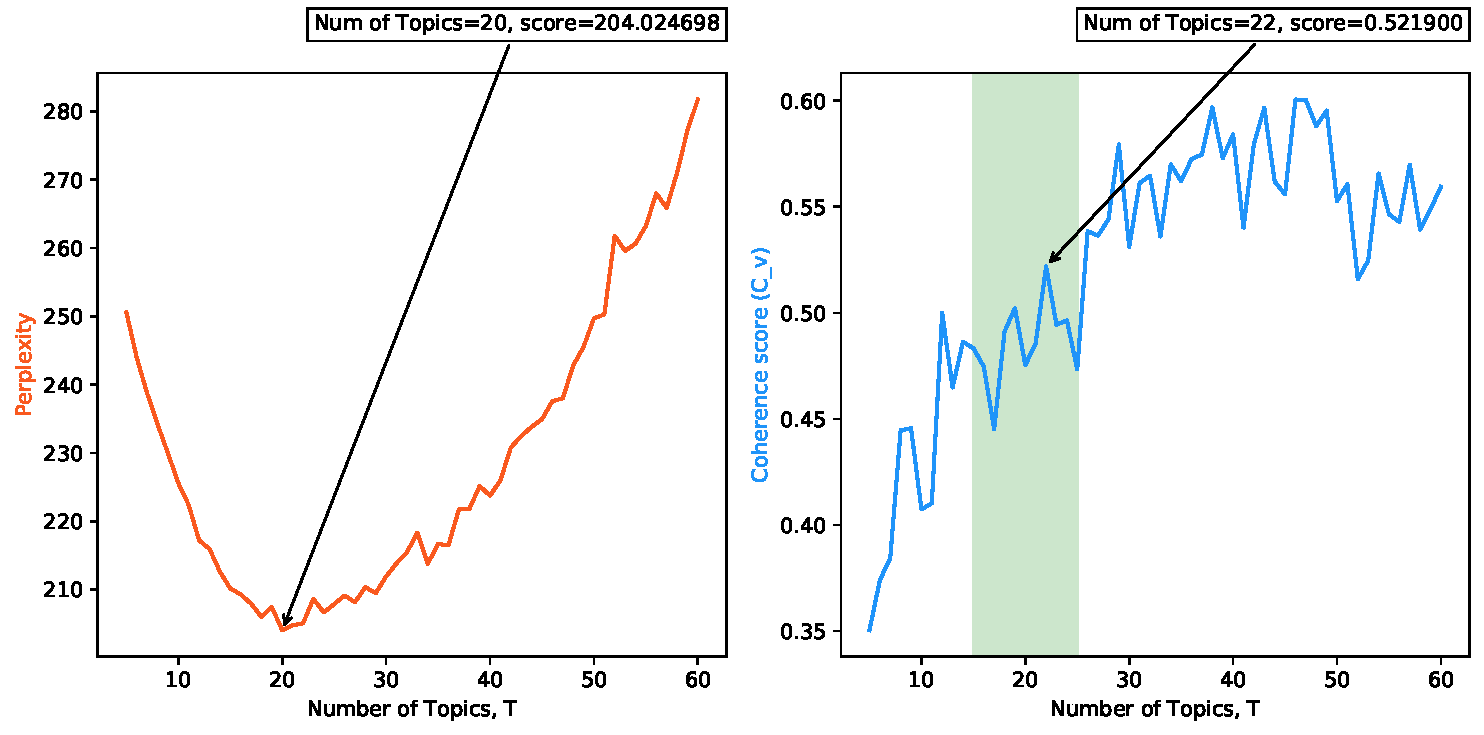
\includegraphics[width=0.9\linewidth]{images/t_scan_combined_plot.pdf}
	\caption{Perplexity for the topic numbers in the range from 5 to 60 \textbf{on the left} and Coherence score with highlighted interest range between 15 and 25 topics \textbf{on the right}. The plots show the changes of selected metrics with number of topics' growth as well as selection of the best number of topics based on our pipeline}
	\label{fig:topic-num}       
\end{figure}

Perplexity is an intrinsic measure, defined as the test sample's as a normalized inverse probability of a test set(\ref{eq:perplexity}), indicating how badly a model predicts held-out documents.
Consider for example \footnote{this is a simplified example for illustration only, the actual DTM language model used in this paper does evaluate sentences to predict the next word, but uses a bag of words model} the sentence "2020 was a year of many ......".
A plausible replacement for "....." would be "changes" or "difficulties". Not so plausible replacements would be "rhinoceroses", "recumbentibuses", "yogeybogeyboxes" etc. If a registers a word in a document it does not expect (e.g. does not place a high probability of occurrence in), it is "perplexed".
Considering the unseen "test data set" was not used in models training process, the best model is the one with the test sample's lowest \textit{Perplexity}. In other words, a low Perplexity score shows that a model is not \textit{perplexed} by unseen test data, thus has a good understanding of the underlying - "true" language model.

\begin{equation}
    \label{eq:perplexity}
    PP_{of test set}(W) = \sqrt[N]{\frac{1}{P(w_1, w_2, ... , w_n)}}
\end{equation}

In addition to \textit{Perplexity} we consider \textit{Coherence} score\cite{ref_lda_coh_exploring} \cite{ref_lda_coh_1} \cite{ref_lda_coh_2} \cite{ref_lda_coh_3}. Since \textit{Perplexity} is a function of likelihood and Chang et al.\cite{ref_lda_human_evaluation} challenge the sole usage of the likelihood for evaluation of topic modeling .
\textit{Coherence} scores try to automatically model human interpretability of topics, that is, trying to predict how intuitively coherent a topic would be perceived as by a human interpreter. 
A set of elements is coherent if the elements in support each other.
For example a topic with a top word count of "lollipop, x-ray, exhaust fumes, melancholy, Christmas", while poetically interesting, would likely be perceived as less coherent than one that has the words "mine, mining, ore, copper, gold" as the top results.
A good coherence measure would mirror a human scoring as close as possible.
In this paper we utilize a compound coherence measure called $C_v$ which has been proposed by Roeder et al.\cite{ref_lda_coh_exploring}, however any other coherence measure would be possible.
The reason we chose Roeder's V-measure is that it showed the highest correlation with human scoring.
In their unified framework, every coherence measure including the  $C_v$ we chose is formally the cross product of four sub component: $C_v  = S^{one}_{set} \times P_{sw(110)} \times \bar{m_{cos(nlr,1)}} \times \sigma_a$ where $S$ is the segmentation and formally:
$S^{one}_{set} = \Big\{ (W', W*) | W' = {w_i}; w_i \in W; W* = W \Big\}$
$P$ is the word probabilities and  $P_{sw(110)}$ refers to a Boolean sliding window word count with a sliding window of a length of 110. 
$M$ is the confirmation measures and $\bar{m}_{cos(nlr,1)}$ is the cosine vector similarity between the (direct) normalized log ratio measure and 1.
$\sigma_a$ is simply the arithmetic mean

The exact measure used is essentially an implementation choice and other measures like Rate of Perplexity changes (RPC) \textb{todo: reference to RPC paper} Absolute Perplexity\textb{todo: reference to AP paper} are possible and could inform the number of topics. In this case, we have decided to use the $C_v$ measure on the basis of human correlation.

\begin{table}[h!]
\centering
\caption{Scan for T}\label{tabl_scan_for_t}
\begin{tabular}{l|c|c|c|c|c|c|c|c|c|c}
\hline
\textbf{T} & 5 & 6 & 7 & 8 & 9 & 10 & 11 & 12 & 13 & 14 \\ 
\hline
\textbf{Coherence score}  & 0.3503 & 0.3739 & 0.3844 & 0.4446 & 0.4456 & 0.4073 & 0.4102 & 0.5000 & 0.4648 & 0.4863 \\ 
\textbf{Perplexity score} & 250.5926 & 243.9091 & 238.7075 & 234.1842 & 229.9378 & 225.5807 & 222.3518 & 217.1879 & 215.9270 & 212.6003 \\ 
\hline
\textbf{T} & 15 & 16 & 17 & 18 & 19 & 20 & 21 & 22 & 23 & 24 \\ 
\hline
\textbf{Coherence score}  & 0.4833 & 0.4747 & 0.4451 & 0.4911 & 0.5022 & 0.4753 & 0.4857 & 0.5219 & 0.4944 & 0.4964 \\ 
\textbf{Perplexity score} & 210.1390 & 209.2814 & 207.9078 & 205.9856 & 207.4184 & 204.0247 & 204.7330 & 205.0455 & 208.6151 & 206.6435 \\ 
\hline
\textbf{T} & 25 & 26 & 27 & 28 & 29 & 30 & 31 & 32 & 33 & 34 \\ 
\hline
\textbf{Coherence score}  & 0.4734 & 0.5385 & 0.5364 & 0.5441 & 0.5794 & 0.5311 & 0.5612 & 0.5647 & 0.5360 & 0.5700 \\ 
\textbf{Perplexity score} & 207.8502 & 209.1074 & 208.1385 & 210.3430 & 209.4555 & 211.9088 & 213.8270 & 215.4486 & 218.3048 & 213.7529 \\ 
\hline
\textbf{T} & 35 & 36 & 37 & 38 & 39 & 40 & 41 & 42 & 43 & 44 \\ 
\hline
\textbf{Coherence score}  & 0.5621 & 0.5725 & 0.5747 & 0.5969 & 0.5729 & 0.5842 & 0.5402 & 0.5796 & 0.5967 & 0.5619 \\ 
\textbf{Perplexity score} & 216.6616 & 216.4665 & 221.7208 & 221.7515 & 225.1433 & 223.7432 & 225.9876 & 230.7841 & 232.4538 & 233.8112 \\ 
\hline
\textbf{T} & 45 & 46 & 47 & 48 & 49 & 50 & 51 & 52 & 53 & 54 \\ 
\hline
\textbf{Coherence score}  & 0.5559 & 0.6006 & 0.6004 & 0.5880 & 0.5954 & 0.5527 & 0.5607 & 0.5159 & 0.5246 & 0.5657 \\ 
\textbf{Perplexity score} & 234.9321 & 237.5685 & 237.9971 & 242.7622 & 245.5376 & 249.7083 & 250.2801 & 261.7780 & 259.5916 & 260.6373 \\ 
\hline
\textbf{T} & 55 & 56 & 57 & 58 & 59 & 60 & 61 & 62 & 63 & 64 \\ 
\hline
\textbf{Coherence score}  & 0.5465 & 0.5429 & 0.5699 & 0.5393 & 0.5489 & 0.5595 \\ 
\textbf{Perplexity score} & 263.2336 & 268.0206 & 265.8926 & 271.0284 & 277.2224 & 281.7555 \\ 
\end{tabular}
\end{table}

\textbf{Todo: Add it as an algorithm}
We construct our automated pipeline to choose a value of $T$, in the following way. We sample all documents for the first time slice in the corpus and iteratively calculate the coherence and perplexity scores for $T$ in the range between 10 and 60. As we state above for practical reasons we choose to compute logarithm of the Perplexity score as normalized likelihood and Coherence measure called $C_v$. We found a global maximum for \textit{log}(Perplexity) at -7.672555 and the corresponding $T$ equal to 20. As the second step, we define an interest area as $T$ +- 5 of a \textit{log}(Perplexity score) global maximum. And fine-tune the $T$ in the range by searching for the maximum Coherence $C_v$ score within that interest area. We found interest area's maximum maximum Coherence $C_v$ at 0.521899 and corresponding $T$ equal to 22.
Values are shown in Table \ref{tabl_scan_for_t}.

\subsubsection{Topics distribution, variation and run parameters}
Three other run parameters are $\alpha$ $\beta$ and $\sigma$  as well as the minimum number and maximum number of iterations. 
$\alpha $ is the Dirichlet prior of the topic proportions $\theta$, we chose the default value of 0.01. $\beta$ is the Dirichlet prior of the word distributions, we chose the default parameter of 0.5.
In general we have noticed that the choice of $\alpha$ and $\beta$ is less important, as the model converges after a sufficient number of iterations for any $\alpha$ and $\beta$. For this reason we do not develop an automated solution here but instead use the default values which were heuristically developed by Blei and al.

Of greater importance is $\sigma$, which signifies the allowed variation of $\beta$ between time slices. $\sigma$ controls how much the topics themselves, being distributions over words, are allowed to vary from year to year.
Choosing $\sigma$ too low will make the topics static and not utilize the dynamic nature of the DTM model, choosing it too high will evolve the topics beyond recognition after a few time slices.
After some experimentation we also choose to keep the default value of 0.005, which seems to give an intuitively plausible topic drift. 
We instruct the model to use a minimum and maximum number of iterations of 5 and 30 respectively in the variational inference algorithm.

\subsection{Extraction of Risk Factors}
Using variational inference we have inferred two posterior distributions: the distribution of words over the vocabulary per topic $\vec{\phi}$, and distribution of topics in the individual documents $\theta$. By utilizing the DTM algorithm we arrive at these two distributions for every time slice we have.
The word distribution represented by a vector of length $n$, where $n$ is the number of words in the vocabulary. The list of top five words for every topic and the corresponding shift over the experiment time frame is displayed in Appendix I. 
Distribution of topics in the individual documents is represented by a vector of length $T$, where $T$ is the number of topics. The distribution of topics in the individual documents is crucial for this paper. Each document belongs to exactly one company and one year and is split into a distribution of $T$ topics.

We group documents by company and compute the unweighted arithmetic average of the topic distribution for all the documents (that is 10-K and 10-Q) of one company within one year. Every company is now represented by a T-dimensional vector on a simplex, where $T$ is the number of topics. This T-dimensional vector changes every year, as the DTM recomputes the topic distribution  the vector will wander over the simplex.

Figure\ref{fig:3-companies-topics-distribution} shows example of a such distribution for three companies.

\begin{figure}
    \centering
	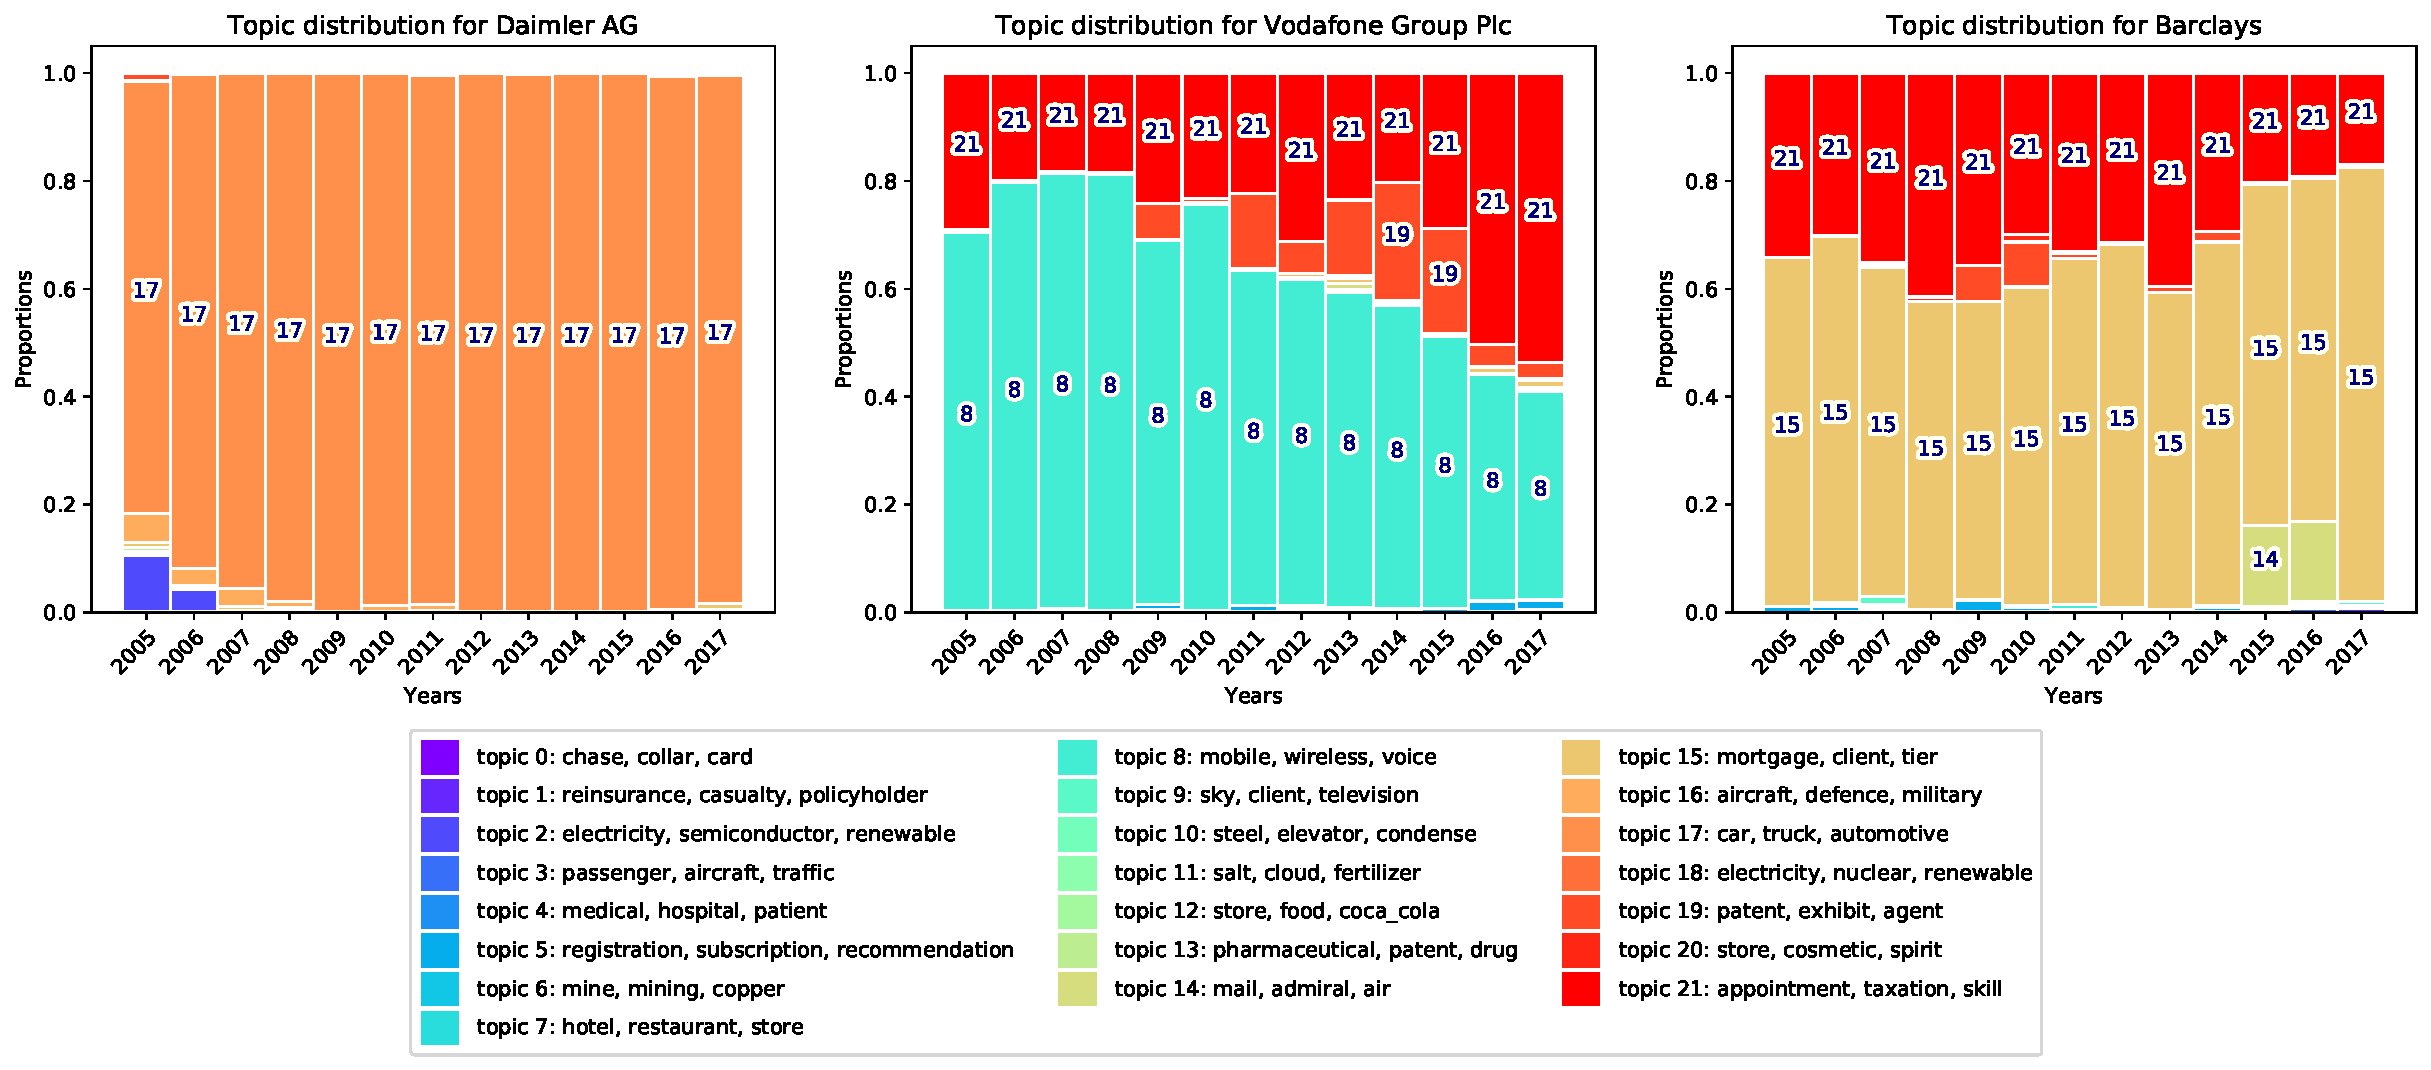
\includegraphics[width=\linewidth]{images/3_companies.pdf}
	\caption{Plot of topics distribution for Daimler AG, Vodafone Group Plc and Barclays plc (left to right) over the experiment time frame. Full list of plots available in the appendix sections A-H}
	\label{fig:3-companies-topics-distribution}       
\end{figure}
The stock vectors span a vector space of $T$ dimensions, with the entries representing the composition of the stock into the topic dimensions.

Our goal is now to find an orthonormal basis for this vector space, in other words, to isolate the individual topic components.

For this we combine the  row vectors to form a matrix .
The new orthonormal basis will be the vectors which have 1  in one entry and 0 in all the others, for example:

$[1,0,0, ... , 0,0]$ or $[0,0,1,..., 0,0]$

This vector represents a pure topic vector, as the entire distribution is concentrated in a single topic.

As we currently only have company topic vectors, which have a variety of entries in the $T$ topics, we now want to find the coefficient vectors $\vec{x_1}, \vec{x_2}, \vec{x_3}, ... \vec{x_n}$  needed to combine the vectors in such a way that they form the orthonormal basis vectors $\vec{b_i}$.

For this, we need to approximately solve the linear equation:

$$\Theta w = b$$

once for each basis vector.

Since the number of stocks usually exceeds the number of topics, the number of independent equations will exceed the number of unknowns. The matrix  will have more rows than w has entries.

The system will thus be in general be overdetermined and can thus be only approximately solved.

In order to find a suitable combination of weights we thus use a python implementation of the least-squares algorithm to a linear matrix equation. The implementation is a part of the NumPy library. The solution returns by \textit{numpy.linalg.lstsq}\cite{ref_linalg_numpy} function.


The extracted coefficients $(w_1, w_2, w_t)$ are then used to decompose stock returns into components.

This equation fitting will have to be redone at the end of each year, as the data for the new time slice changes the topic distribution for each company. 

\section{Technical Caveats when setting up the the experiment}

1) No. of stocks vs. No. of topics - the more reports are there in the data set , the better the intuitive interpretability of the topics becomes. A static LDA model will in general need less reports to give a good interpretability of topics, while with the dynamic topic model used in this paper more reports are necessary. For the dynamic approach to work, the ideal data set should be maybe three or four times as large as the number of topics.
\\
2) Extreme weightings - If the number of stocks is too small compared to the number of topics, extreme weighting in the portfolio will occur. These cannot be used to construct meaningful financial portfolios, as they would imply excessive leverage.
\\
3) Time series of reports - exit and entry of new stocks in the data space will significantly influence the composition of topics. It is therefore recommended to use a data set of stable and established companies for the construction of indices. Companies with too short of a time horizon should be eliminated.
\\
4) Type of report - different reports, such as the 10- K and 10-Q  reports consistently show somewhat different topic profiles, it may therefore be  more stable to use only one type of report


\section{Observations} 
\textbf{Topic Proportions}
We graph the computed topic proportions in Appendix C of this paper.
The first observation we can make is that the topic proportions of companies is surprisingly stable. 
Most company's proportions remain very similar over time, meaning that the "topic fingerprint" of the texts does not change much. While some companies show a drift in topic proportions, we do not see discontinuous jumps.
The topic allocations also seem very plausible, with companies like Lufthansa dominated by Topic 3: "passenger, aircraft, traffic", Daimler and BMW by Topic 17: "car, truck, automotive", Procter and Gamble by topic 13: "pharmaceutical, patent, drug" and LMVH dominated by Topic 20: "store, cosmetics, spirit".
There are some topics in which the algorithm seems to have difficulty disentangling words with multiple semantic meanings, such as the Topic 11: "salt, cloud, fertilizer", which drifted from a topic talking about physical clouds to more metaphorical digital clouds.
One conspicuous feature is the presence of the more accounting related topic 21: "appointment, taxation, skill" in a lot of companies.
While we are not able to map this to any , it is perhaps not surprising that company accounting reports devote a significant portion to accounting and taxation matters.


\textbf{Topic Indices}
From the topic proportions we extract weights for pure topic indices via change of basis, as described above.

In order to contextualize the indices we have created , we map each of the indices, if possible, to a existing tradable industry index:

\begin{table}[!ht]
  \begin{center}
    \caption{Topic to Industry Index Mapping}
    \begin{tabular}{l|c|r}
      \textbf{Topic No.} & \textbf{Topic Index} & \textbf{Benchmark Index}\\
      \hline
      Topic 0 & "chase, collar, card, mortage ..." & XLF Financial Select Sector SPDR Fund \\
      Topic 1 & "reinsurance, casualty, policyholder" & KIE SPDR S\&P Insurance ETF \\
      Topic 2 & "electricity, semiconductor, renewable" & XLK Technology Select Sector SPDR Fund \\
      Topic 3 & "passenger, aircraft, traffic, cargo, air ..." & XTN SPDR S\&P Transportation ETF\\
      Topic 4 & "medical, hospital, patient, preference, dialysis ..." & XHS SPDR S\&P Health Care Services ETF \\
      Topic 5 & "registration, subscription, recommendation" & --- \\
      Topic 6 & "mine, mining, copper, gold, ore ..." & XME SPDR S\&P Metals and Mining ETF \\
      Topic 7 & "hotel, restaurant, store, travel, club, premier ..." & PEJ Invesco Dynamic Leisure and Entertainment ETF \\
      Topic 8 & "mobile, wireless, voice, operator ..." & XLC Communication Services Select Sector SPDR Fund \\
      Topic 9 & "sky, client, television, advertising, consumer..." & ---- \\
      Topic 10 & "steel, elevator, condense, stainless, raw ..." & XHB SPDR S\&P Homebuilders ETF \\
      Topic 11 & "salt, cloud, fertilizer, potash magnesium ..." & XLB Materials Select Sector SPDR Fund \\
      Topic 12 & "store, food, coca-cola, bottle ..." & XLP Consumer Staples Select Sector SPDR Fund \\
      Topic 13 & "pharmaceutical, patent, drug, adhesive, patient..." & XLV Health Care Select Sector SPDR Fund \\
      Topic 14 & "mail, admiral, air, logistic, car" & XLI Industrial Select Sector SPDR Fund \\
      Topic 15 & "mortgage, client, tier, card, branch ..." & XLRE The Real Estate Select Sector SPDR Fund  \\
      Topic 16 & "aircraft, defence, military, space, engineering ..." & XAR SPDR S\&P Aerospace \& Defense ETF \\
      Topic 17 & "car, truck, automotive, bus, engine, marketable ..." & CARZ First Trust NASDAQ Global Auto Index Fund \\
      Topic 18 & "electricity, nuclear, renewable, emission" & XLE Energy Select Sector SPDR Fund \\
      Topic 19 & "patent, exhibit, agent, pharmaceutical, drug ..." & XHE SPDR S\&P Health Care Equipment ETF \\
      Topic 20 & "store, cosmetic, spirit, woman, luxury ..." & XLY Consumer Discretionary Select Sector SPDR Fund \\
      Topic 21 & "appointment, taxation, skill, turnover, undertaking..." & ---- \\
    \end{tabular}
  \end{center} 
\end{table}

We graph these in Appendix J. One problem we are facing is that some benchmarks have a shorter time horizon than the topic index they are supposed to benchmark. In this case we will normalize the benchmark to the level that the topic index had at the time of the benchmark's starting date and then start the benchmark from there.

Given that the weights were arrived at by pure textual analysis, we observe a remarkably good tracking of the benchmark for Topics 1, 2, 4, 7, 13, 14, 15, 17, 18. 

Furthermore, for the indices in Topic 0, 1, 4, 6, 7, 10, 11, 14, 17, 19, 20 we observe a significant outperformance of Topic indices over benchmark indices. 
The two categories overlap in the Topics 1, 4, 7, 14 and 17, which are indices which show good tracking in addition to outperformance.
This may be partly due to transaction costs and fees, which have not been accounted for the in the Topic Index construction.
%\emph{The shift by it self might provide interesting insights:
%word "coal" and "water" is common word for both topics
%the rise of "wind" and "renewable" and decline of "Germany" in the energy topic.
%Using posterior distribution of words over a topic with added continuity we can plot top $x$ words and see a topic evaluation over the observed time frame. Table\ref{tab:top-words} represent words importance shift for topics "energy" and "extraction", id 06 and 18 respectively. }

%Here go correlation plots \ref{fig:correlation_dig_topics}\\
In addition to the comparison to the traded risk indices, we also compute the correlations of the topic indices between each other.
Most of the indices show a relatively high correlation with each other, as they are correlated with the overall market.
An exception are the topic indices 3, 6, 15 and 18.
Out of these, Topic 6 : "mine, mining, copper" is particularly interesting because in addition to the low correlation it shows a relatively strong return and also outperforms its benchmark by several multiples.

%write sentence about relationship to S&P 500 here

Make observations about the performance vis-a-vis traded indices.

\begin{figure}
    \centering
	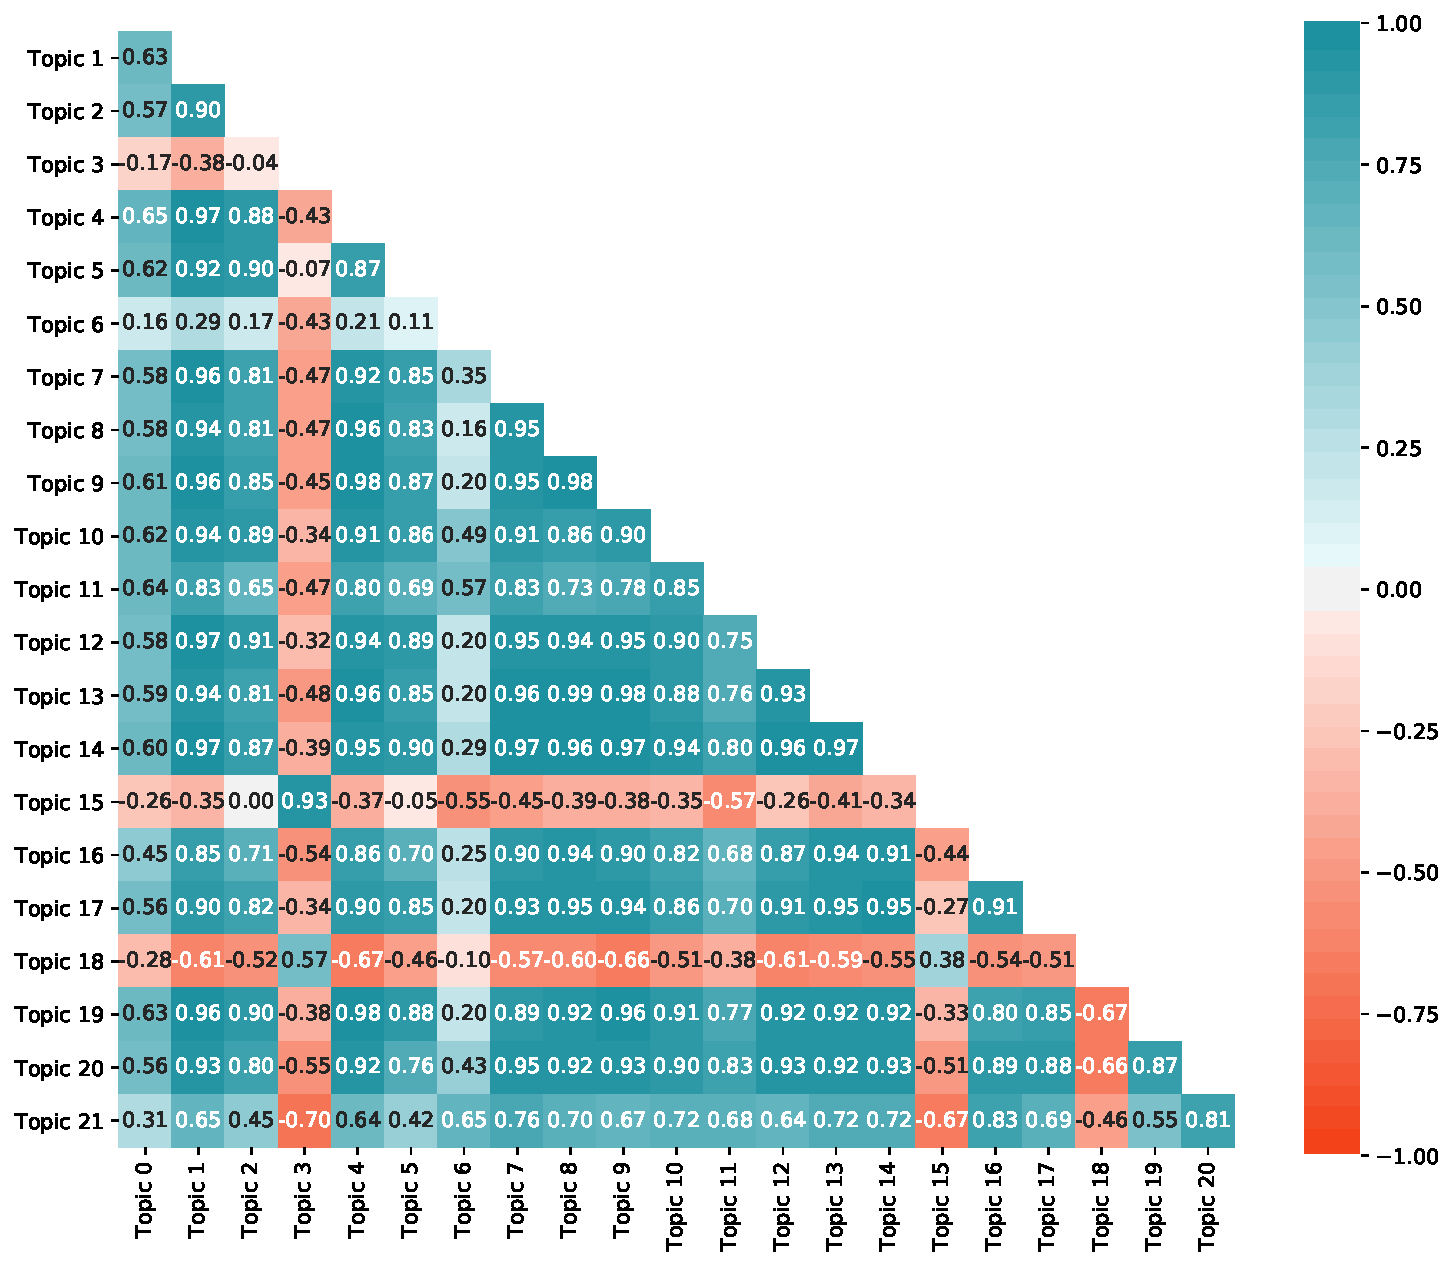
\includegraphics[width=0.9\linewidth]{images/heat_map_correlation_diagonal_topics.pdf}
	\caption{Heatmap of Pearson Correlations between all the topic.}
	\label{fig:correlation_dig_topics}       
\end{figure}

\begin{table}[!ht]
    \centering
    \caption{The shift of word importance in the topic energy on the top and "extraction" on the bottom}
    \label{tab:top-words}
    \resizebox{\textwidth}{!}{
\begin{tabular}{c|c|c|c|c|c|c|c|c|c|c|c|c}
\hline
\textbf{2005} & \textbf{2006} & \textbf{2007} & \textbf{2008} & \textbf{2009} & \textbf{2010} & \textbf{2011} & \textbf{2012} & \textbf{2013} & \textbf{2014} & \textbf{2015} & \textbf{2016} & \textbf{2017} \\ 
\hline
electricity & electricity & electricity & electricity & electricity & electricity & electricity & electricity & electricity & electricity & nuclear & nuclear & nuclear \\ 
water & water & nuclear & nuclear & nuclear & nuclear & nuclear & nuclear & nuclear & nuclear & electricity & electricity & electricity \\ 
nuclear & nuclear & water & water & emission & renewable & renewable & renewable & renewable & renewable & renewable & coal & coal \\ 
emission & emission & emission & emission & coal & emission & coal & coal & coal & coal & coal & renewable & renewable \\ 
coal & coal & coal & coal & renewable & coal & emission & emission & emission & emission & emission & fire & fire \\ 
crude oil & crude oil & crude oil & crude oil & barrel & barrel & barrel & barrel & barrel & barrel & barrel & emission & barrel \\ 
barrel & barrel & barrel & barrel & crude oil & crude oil & upstream & upstream & upstream & tariff & fire & barrel & emission \\ 
station & concession & concession & concession & water & upstream & crude oil & station & station & fire & crude oil & crude oil & crude oil \\ 
concession & station & grid & renewable & concession & concession & station & crude oil & tariff & crude oil & storage & storage & water \\ 
grid & grid & station & station & upstream & station & concession & fire & crude oil & station & station & exploration & storage \\ 
\hline
mine & mine & mine & mine & mine & mine & mine & mine & mine & mine & mine & mine & mine \\ 
gold & gold & copper & copper & copper & copper & copper & mining & mining & mining & mining & mining & mining \\ 
mining & copper & mining & mining & mining & mining & mining & copper & copper & gold & gold & gold & gold \\ 
ore & mining & gold & ore & ore & ore & ore & gold & gold & copper & copper & copper & ore \\ 
copper & ore & ore & gold & gold & mineral & gold & ore & ore & ore & ore & ore & copper \\ 
mineral & mineral & mineral & mineral & mineral & gold & mineral & mineral & mineral & mineral & mineral & exploration & exploration \\ 
exploration & exploration & exploration & exploration & exploration & exploration & exploration & exploration & exploration & exploration & exploration & mineral & mineral \\ 
ounce & ounce & ounce & coal & coal & ounce & ounce & ounce & ounce & ounce & ounce & ounce & ounce \\ 
coal & coal & coal & ounce & ounce & coal & coal & iron ore & iron ore & water & water & water & water \\ 
metal & metal & metal & concentrate & platinum & concentrate & iron ore & coal & water & iron ore & iron ore & underground & pit \\ 
    \end{tabular}
    }
\end{table}

\section{Conclusion}
In this paper we have shown an unsupervised approach of creating thematic topic indices. The main contribution here is to show the possibility of creating indices purely from textual data, without need for human intervention.
Although we have used data from annual and quarterly reports, the approach is not necessarily limited to this, but could also use heterogeneous data sources, such as tweets or news reports.
We believe that the elimination of the need for a human classification system can make the construction of indices less ambiguous and more model based.





\begin{thebibliography}{1}
	\bibitem{BleiJordan2003} D. Blei, A. Ng, M. Jordan,  "Latent Dirichlet Allocation", 2003.
	
	\bibitem{BleiLafferty2006} D.M. Blei, J.D. Lafferty, "Dynamic Topic Modeling", 2006.
	
	\bibitem{Giffiths2006} T.Griffiths, "Gibbs Sampling in the Generative Model of Latent 
	Dirichlet Allocation", 2006
	
	\bibitem{Wang2009}C. Wang, D.M. Blei, D. HeckerMan, "Continuous Time Topic Models",
	2009.
	
	\bibitem{FamaFrench1993} E. Fama and K. French, "Common Risk Factors in the Returns on Stocks and Bonds", 1993.
	
	\bibitem{Curme2013} C. Curme et al, "Quantifying the semantics of search behavior before stock market moves", 2013.
	
	\bibitem{Mukherjee2013} A. Muhkerjee et al, "Exploiting Twitter based Twitter Sentiment for Stock Prediction", 2013.
	
	\bibitem{Ohmura2014} M. Ohmura, Kakusho, Okadome, "Stock Market Prediction by Regression Model with Social Moods", 2014.
	
	\bibitem{chi2012} M. Chi et al, "Construction of Chinese A-shares Network Using Latent Dirichlet Allocation", 2012.
    
    \bibitem{ref_lda_coh_2}
    N. Aletras and M. Stevenson. Evaluating topic coherence using distributional semantics. In Proc. of the 10th Int. Conf. on Computational Semantics (IWCS’13), pp. 13-22, 2013.
    
    \bibitem{ref_lda_human_evaluation}
    J. Chang, J. Boyd-Graber, S. Gerrish, C. Wang, and D. Blei. 2009. Reading tea leaves: How humans interpret topic models. In Advances in Neural Information Processing Systems 21 (NIPS-09), pages 288-296, Vancouver, Canada.
    
    \bibitem{ref_lda_coh_1}
    Jey H. Lau, D. Newman, T.Baldwin. Machine Reading Tea Leaves: Automatically Evaluating Topic Coherence and Topic Model Quality. 14th Conference of the European Chapter of the Association for Computational Linguistics 2014, EACL 2014. 530-539. 10.3115/v1/E14-1056. 
    
    \bibitem{ref_lda_coh_3}
    F. Rosner, A. Hinneburg, M. Ro ̈der, M. Nettling, and A. Both. Evaluating topic coherence measures. CoRR,
    abs/1403.6397, 2014.
    
    \bibitem{ref_lda_coh_exploring}
    M. Röder , A. Both , A. Hinneburg, Exploring the Space of Topic Coherence Measures, Proceedings of the Eighth ACM International Conference on Web Search and Data Mining, February 02-06, 2015, Shanghai, China
    
    \bibitem{ref_finnum_spark}
    A. Spark: BRNIR at the NTCIR-14 finnum task: Scalable feature extraction technique for numeral classification. In: Proceedings of the 14th NTCIR Conference on Evaluation of Information Access Technologies 2019.
    
    \bibitem{ref_Neuhierl_2013}
    A. Neuhierl and A. Scherbina and B. Schlusche: Market Reaction to Corporate Press Releases. In: Journal of Financial and Quantitative Analysis vol. 48, no. 04, 2013. pp 1207–1240
    
    \bibitem{ref_linalg_numpy}
    NumPy: Least Squares solution to linear matrix equation https://numpy.org/doc/stable/reference/generated/numpy.linalg.lstsq.html
    
    \bibitem{ref_ratku_2016}
    A. Ratku and D. Neumann and S. Feuerriegel: Analysis of How Underlying Topics in Financial News Affect Stock Prices Using Latent Dirichlet Allocation. In: 49th Hawaii International Conference on System IEEE Computer Society, Sciences (HICSS) 2016. pp 1072–1081
    
    \bibitem{nltk_book_2009}
    Bird, Steven, Edward Loper and Ewan Klein (2009), Natural Language Processing with Python. O’Reilly Media Inc.
    
    \bibitem{gensim_refernce}
    Rehurek Radim, Gensim Documentation, Release 0.8.6 https://buildmedia.readthedocs.org/media/pdf/gensim/stable/gensim.pdf

    \bibitem{evaluation_10k}
    Travis Dyer, Mark Lang, Lorien Stice-Lawrence,The evolution of 10-K textual disclosure: Evidence from Latent Dirichlet Allocation,Journal of Accounting and Economics, Volume 64, Issues 2–3, 2017, Pages 221-245, ISSN 0165-4101,
\end{thebibliography}
% if have a single appendix:
%\appendix[Proof of the Zonklar Equations]
% or
%\appendix  % for no appendix heading
% do not use \section anymore after \appendix, only \section*
% is possibly needed

% use appendices with more than one appendix
% then use \section to start each appendix
% you must declare a \section before using any
% \subsection or using \label (\appendices by itself
% starts a section numbered zero.)
%


\appendices

\section{Topic distribution for target companies}
\begin{center}
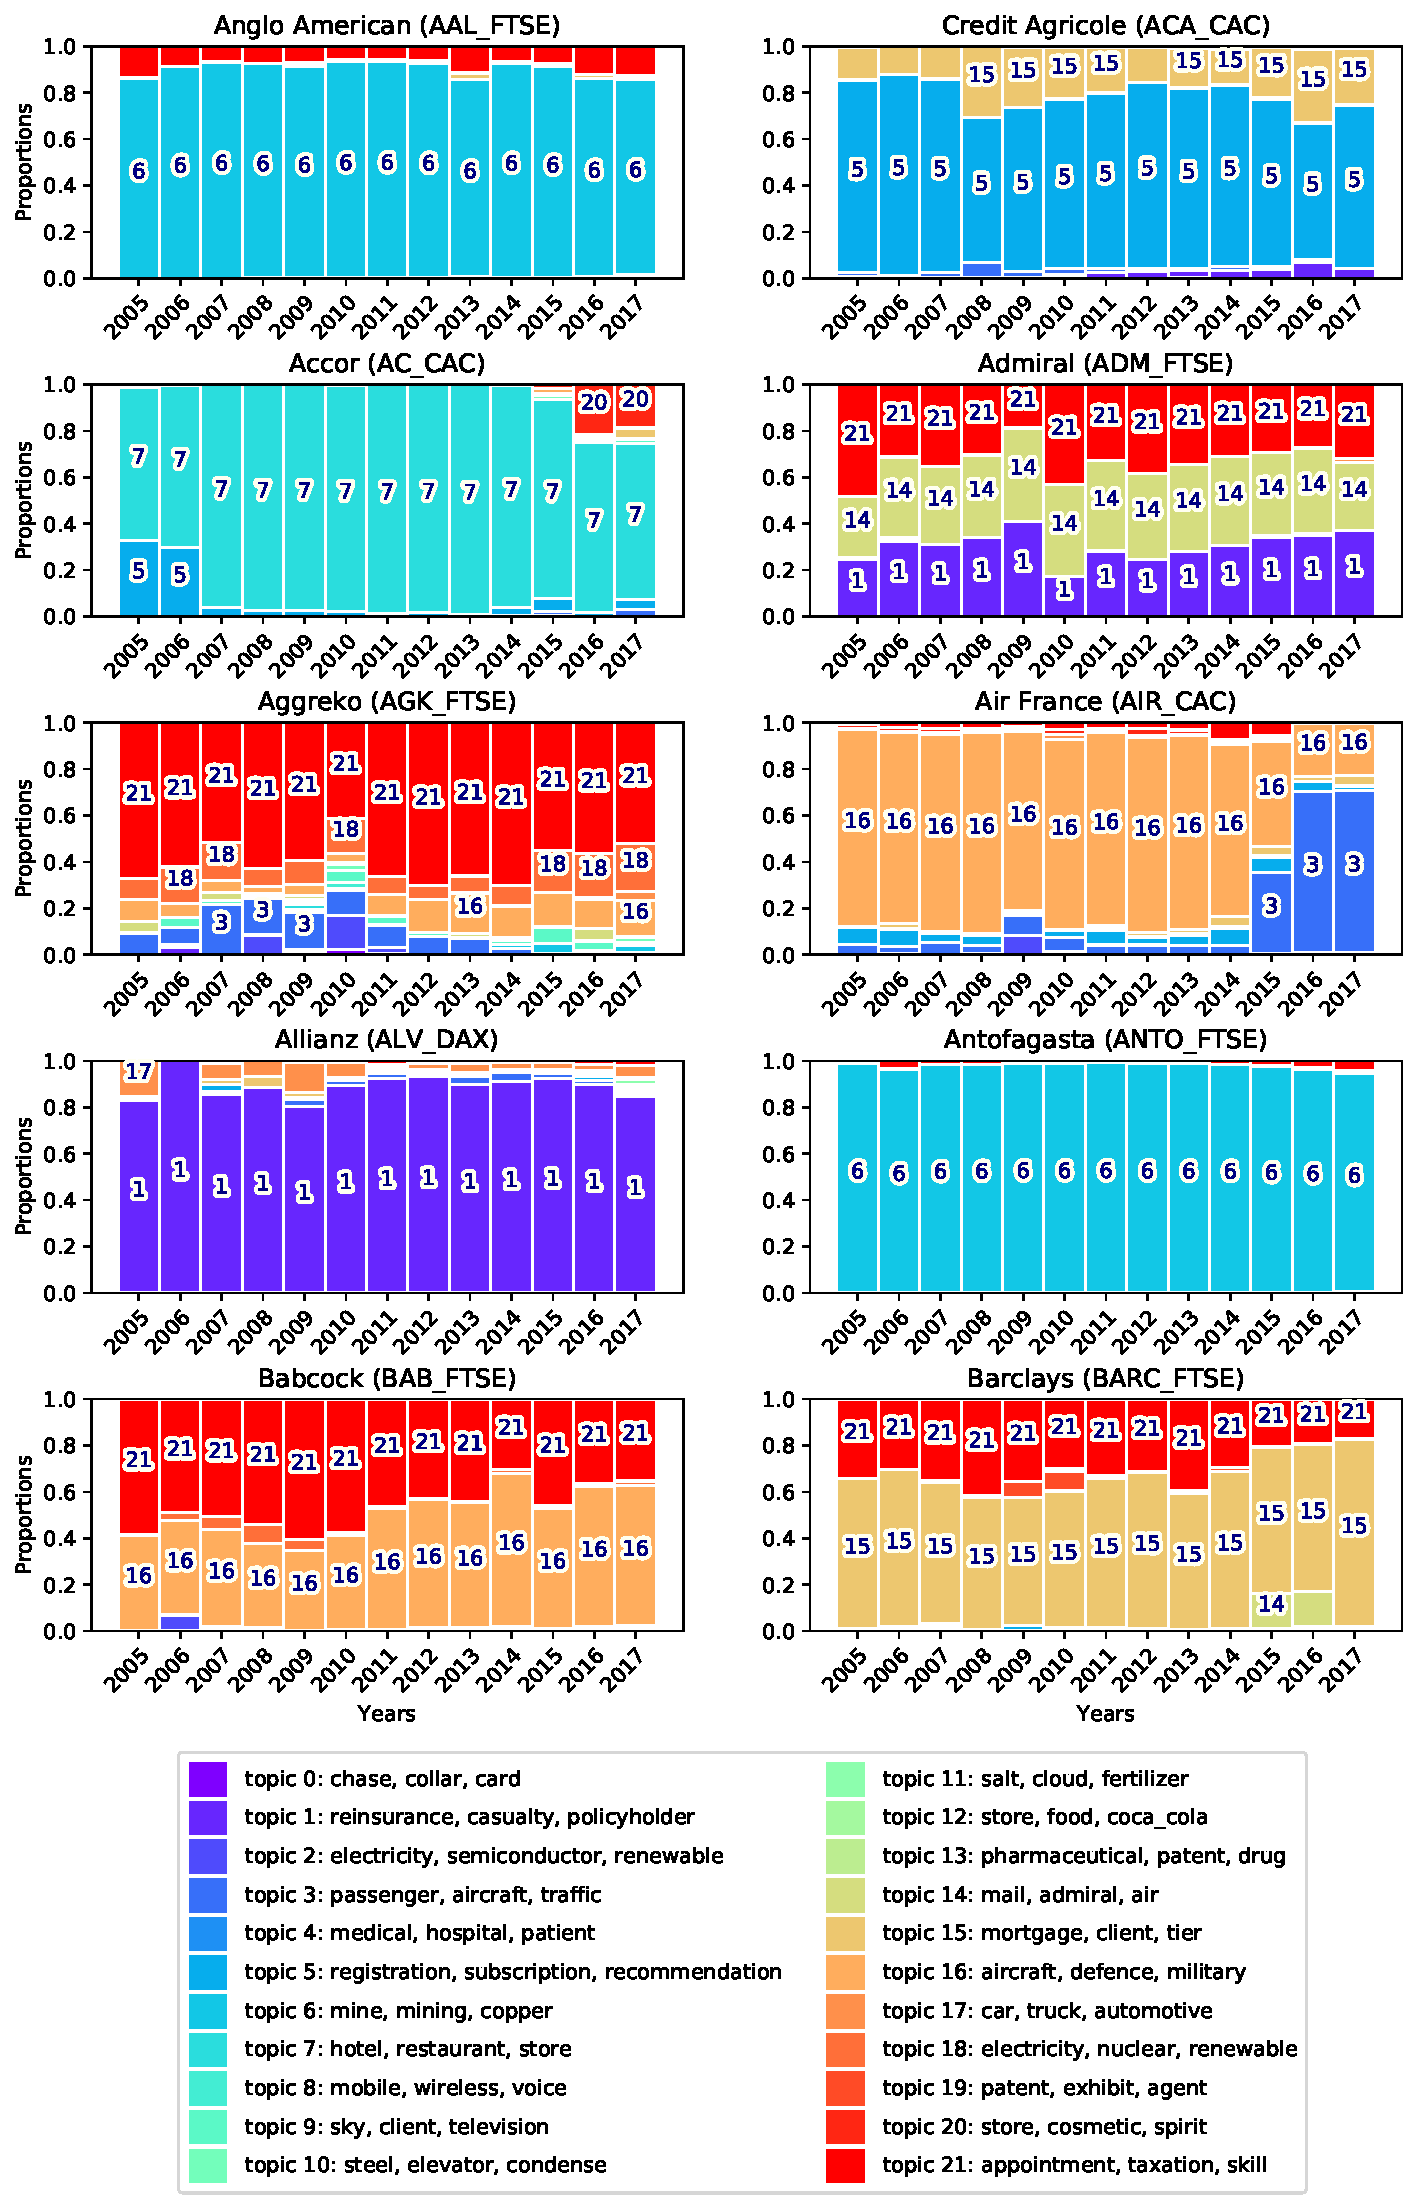
\includegraphics[width=0.85\linewidth]{images/companies_on_page_0.pdf}
\end{center}

\section{Topic distribution for target companies}
\begin{center}
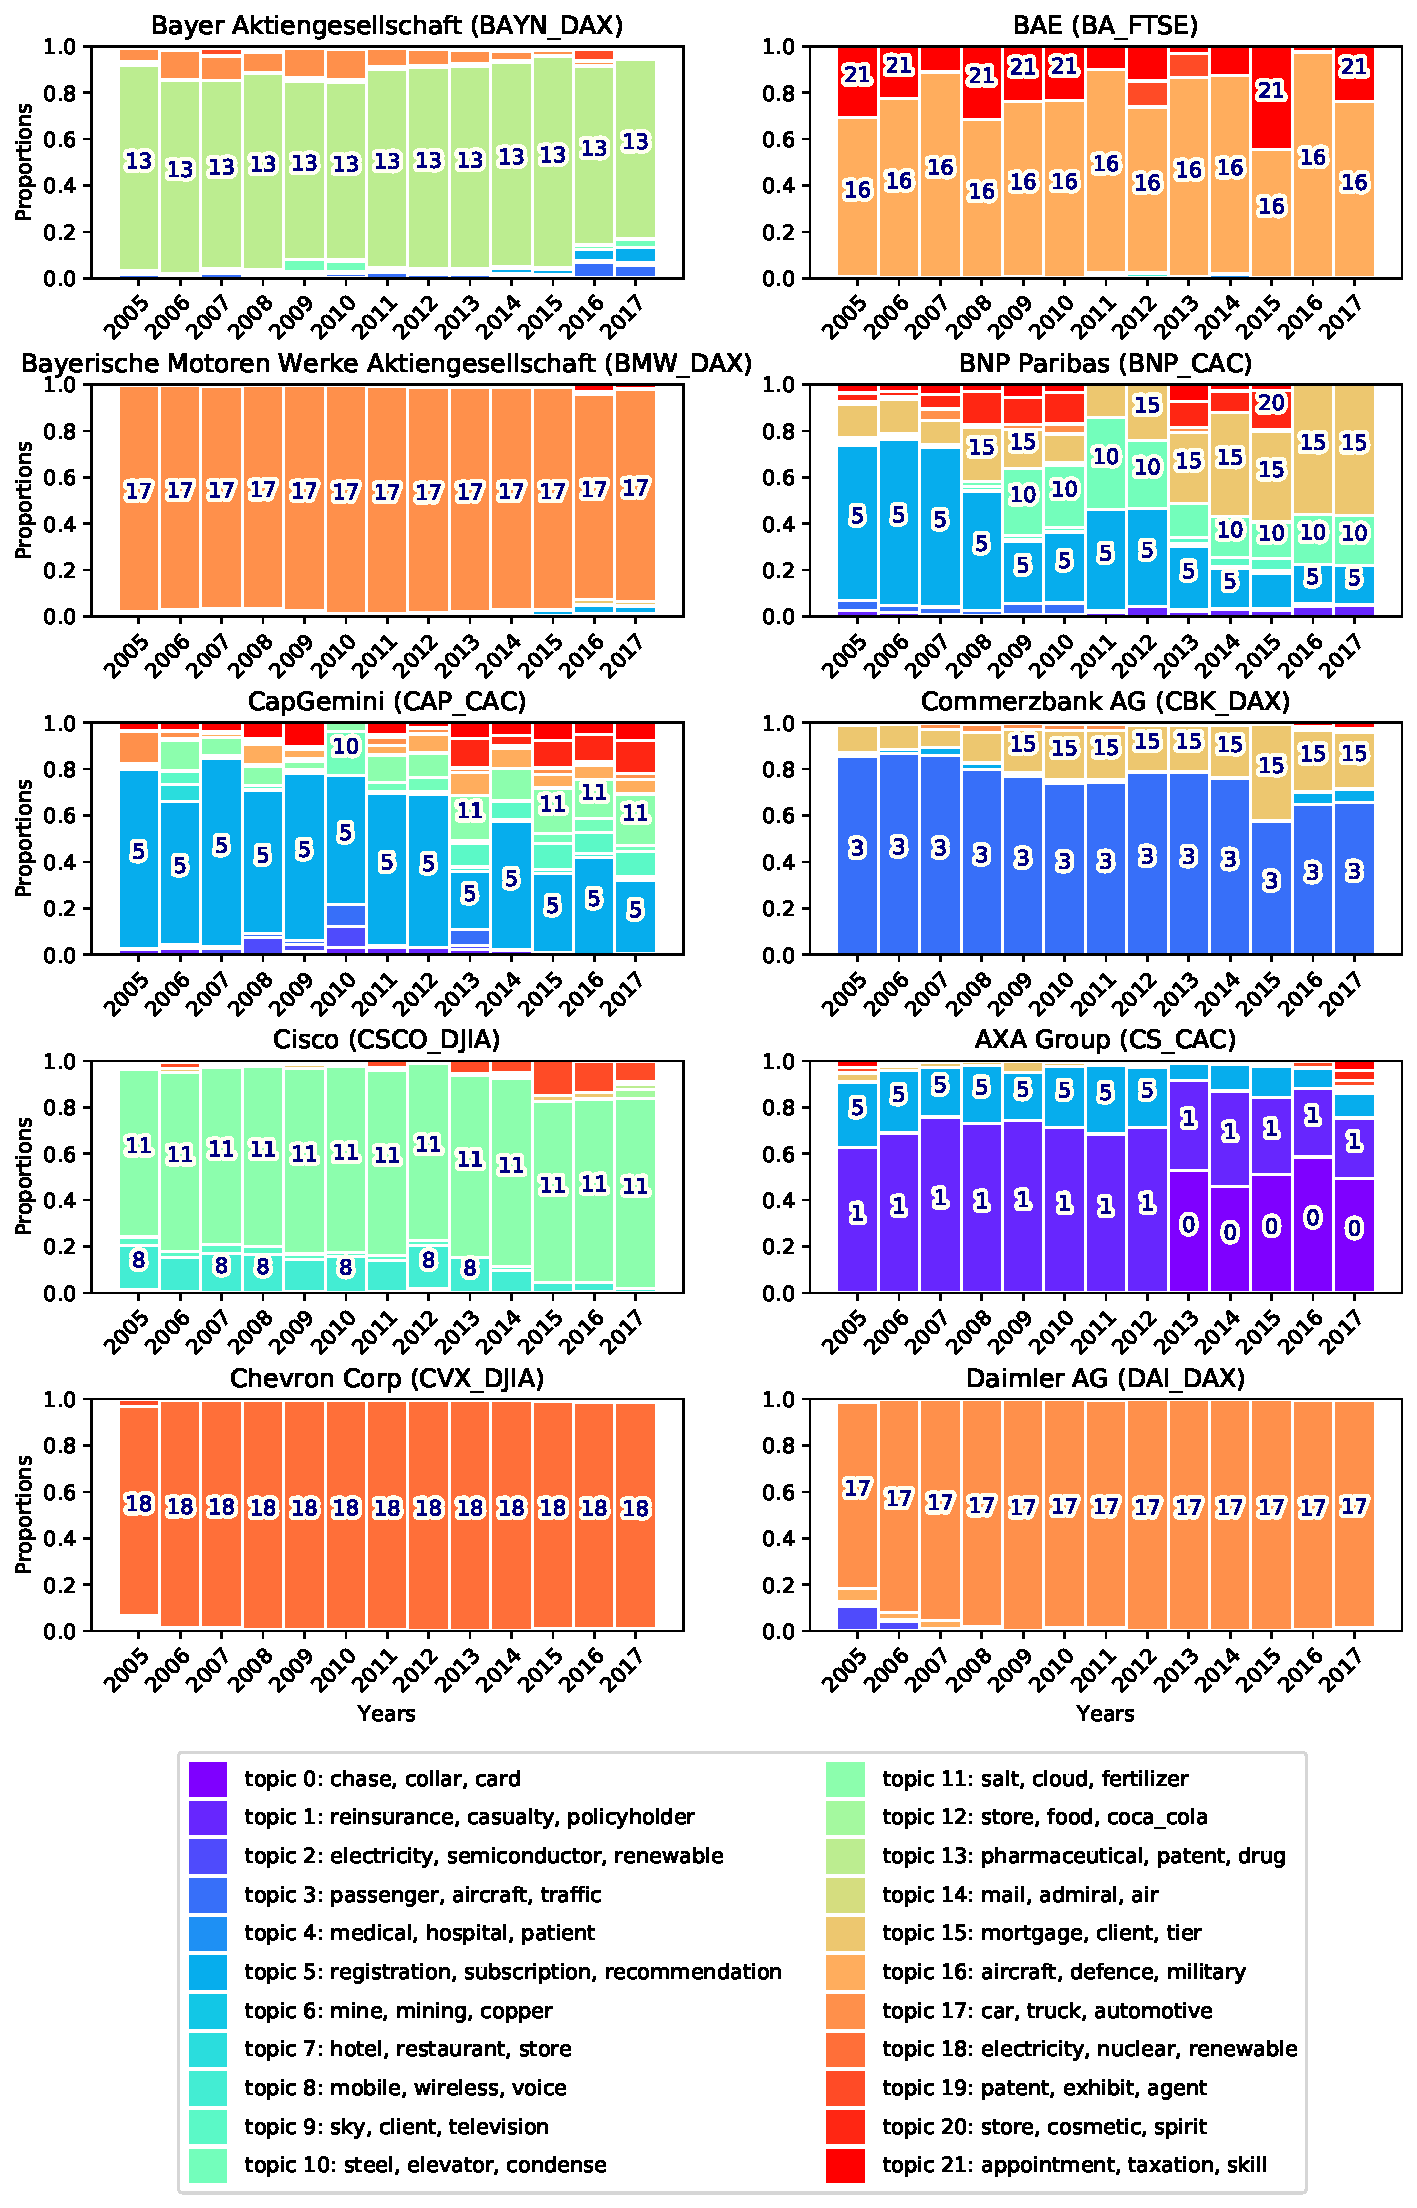
\includegraphics[width=0.85\linewidth]{images/companies_on_page_1.pdf}
\end{center}

\section{Topic distribution for target companies}
\begin{center}
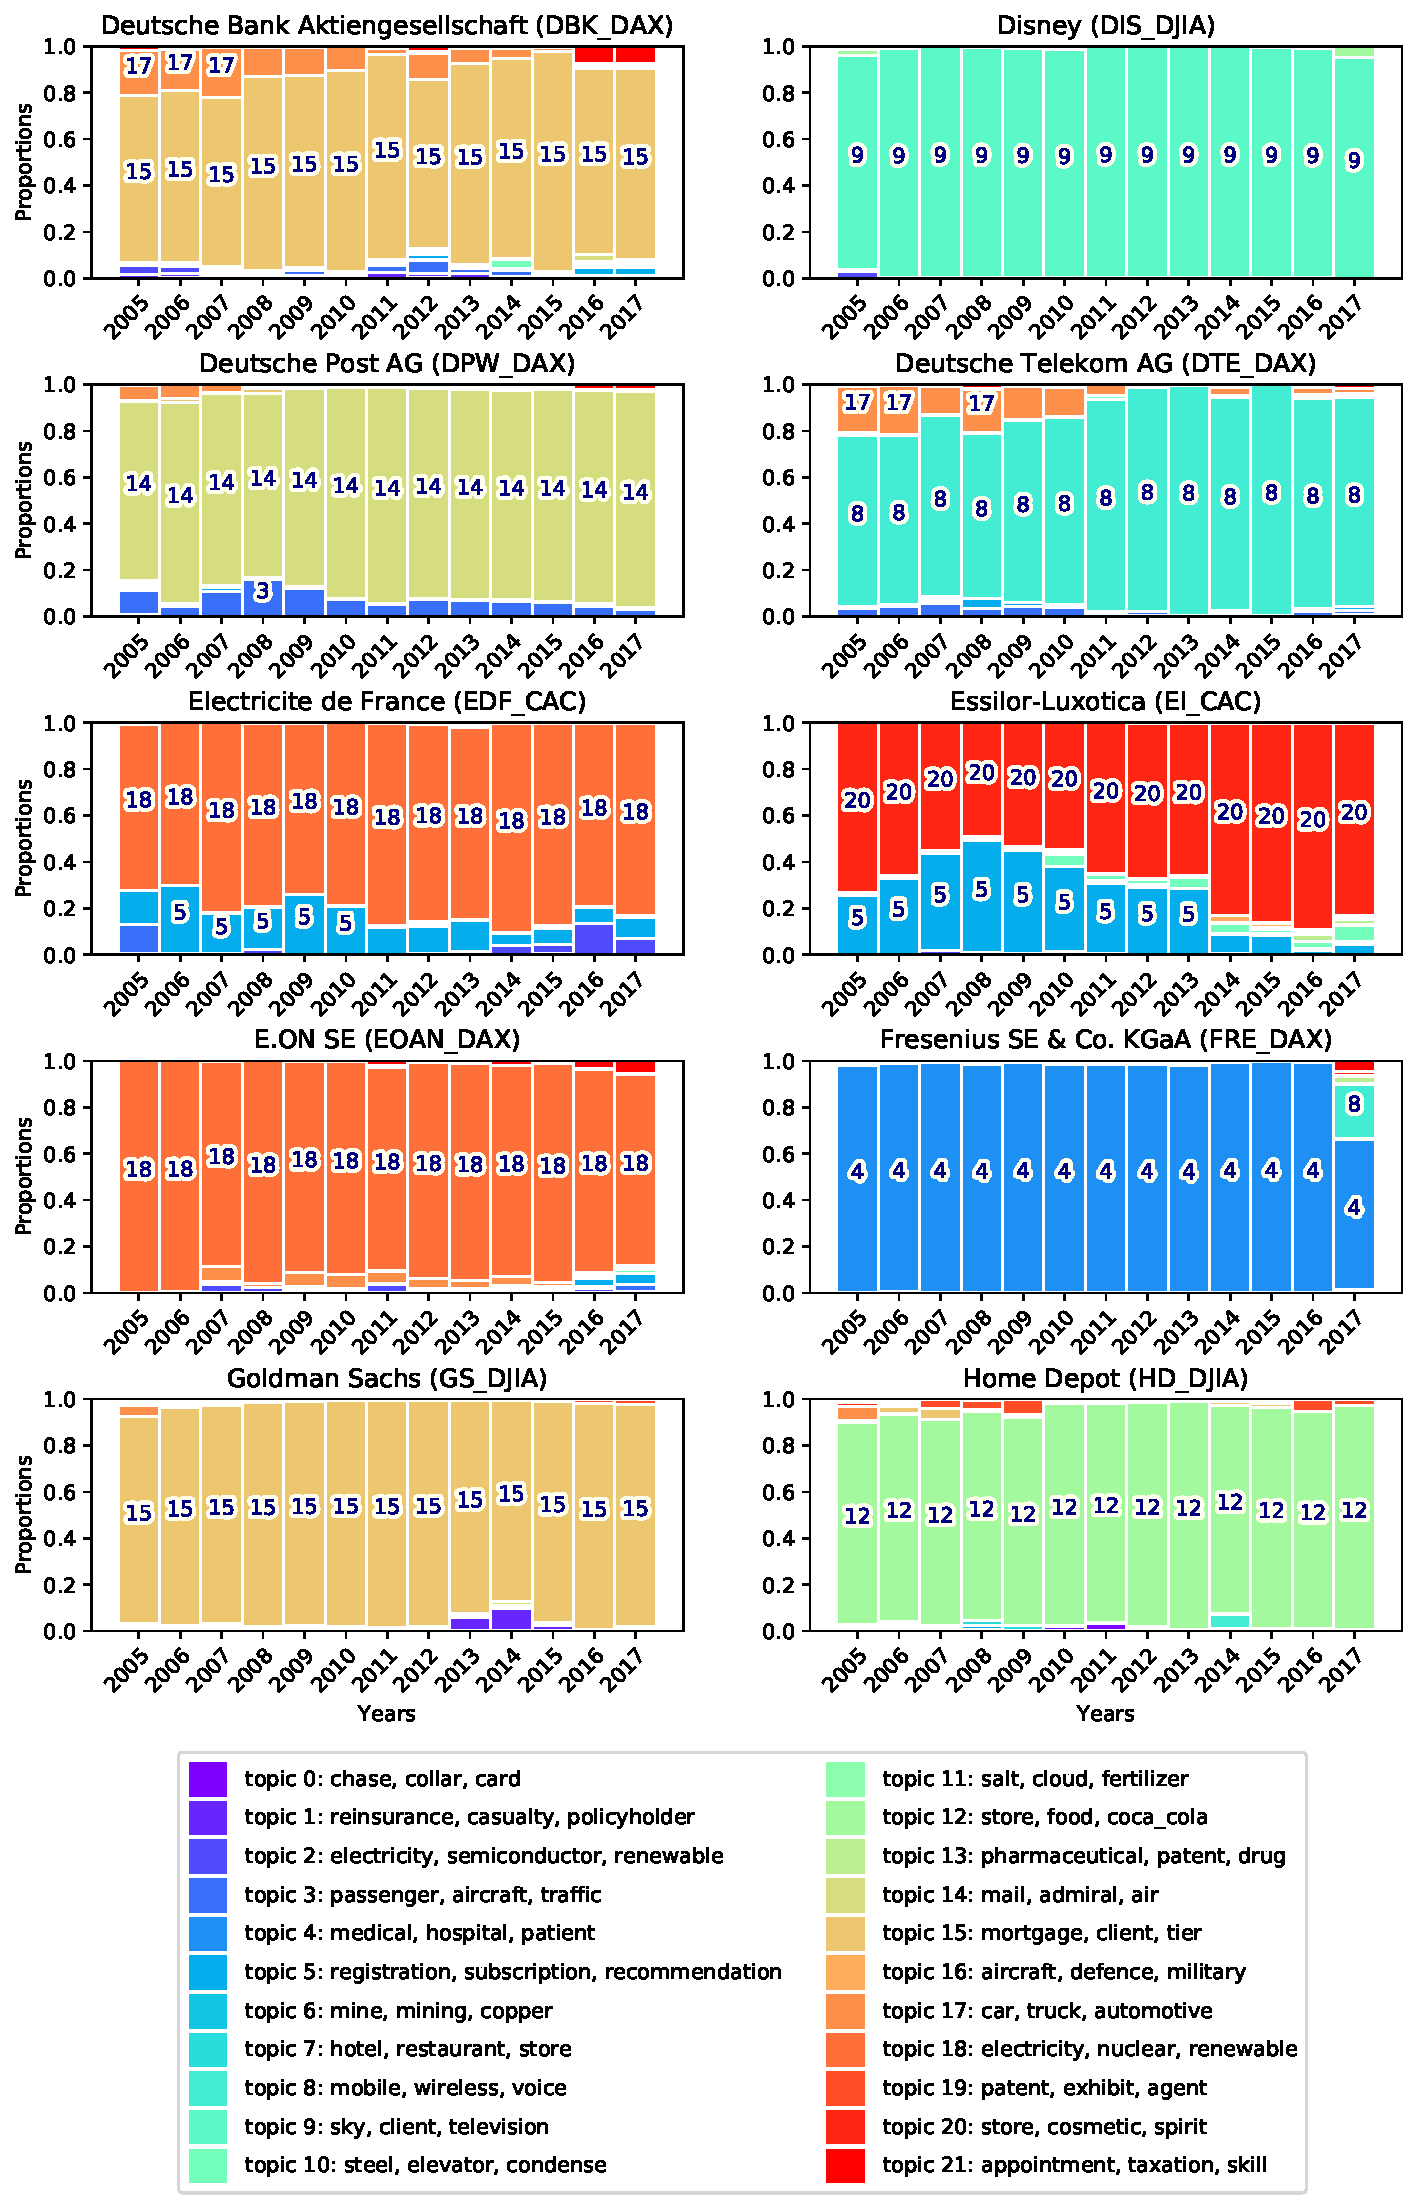
\includegraphics[width=0.85\linewidth]{images/companies_on_page_2.pdf}
\end{center}

\section{Topic distribution for target companies}
\begin{center}
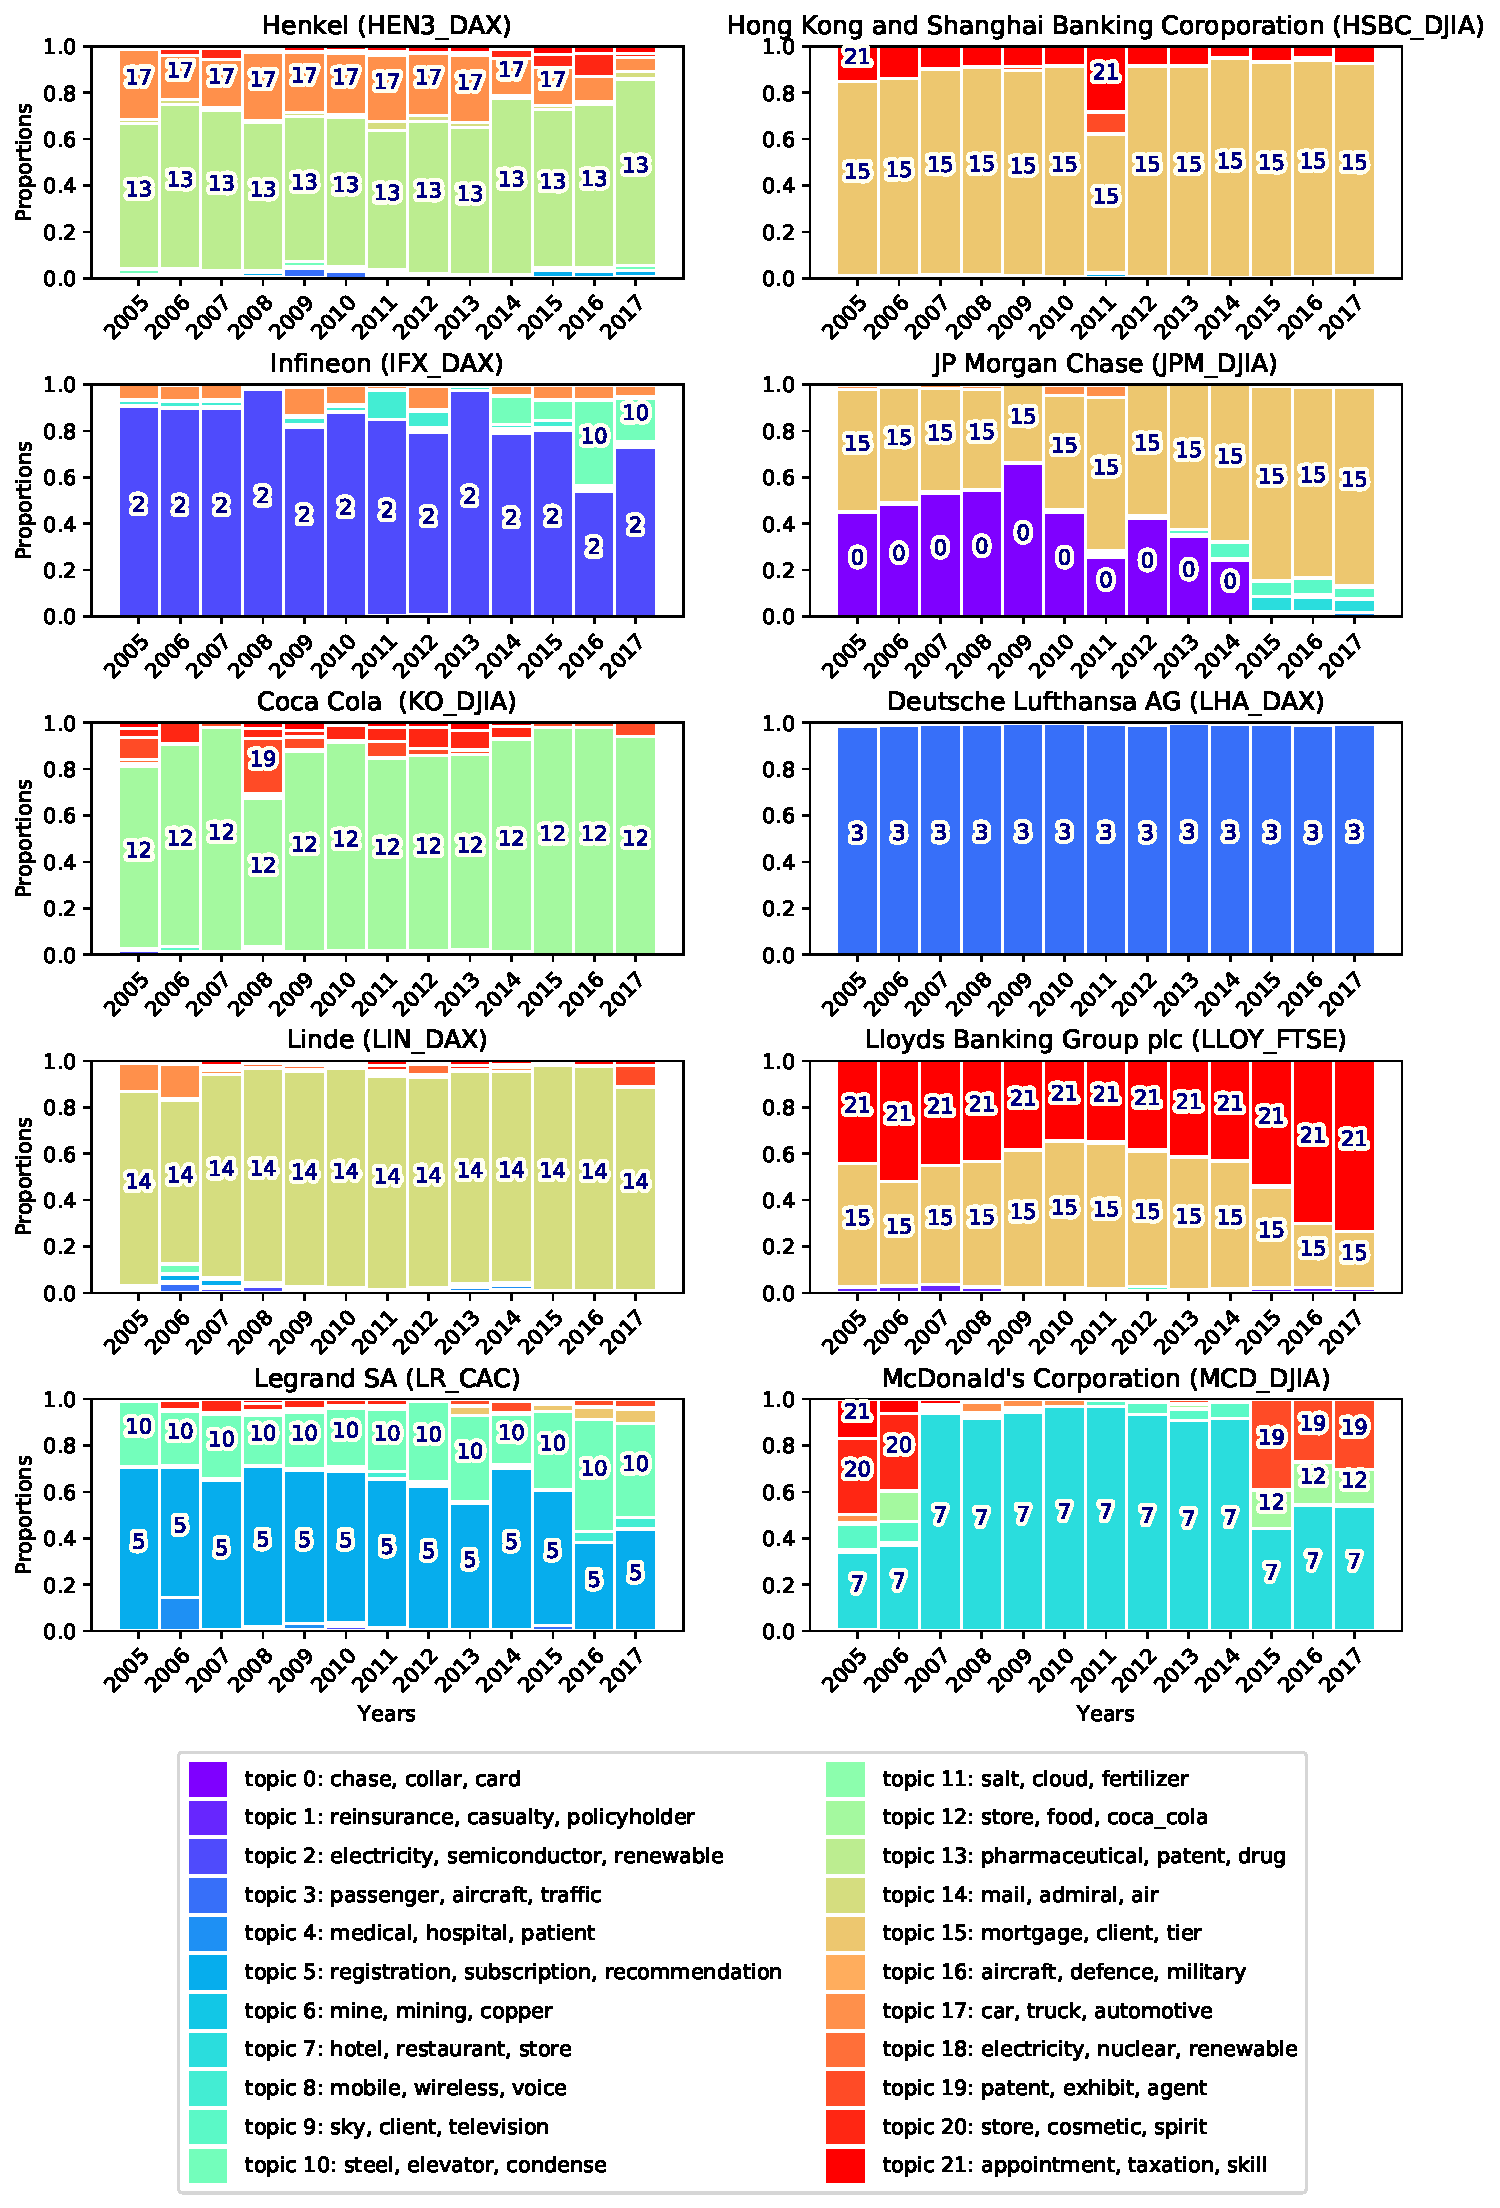
\includegraphics[width=0.85\linewidth]{images/companies_on_page_3.pdf}
\end{center}

\section{Topic distribution for target companies}
\begin{center}
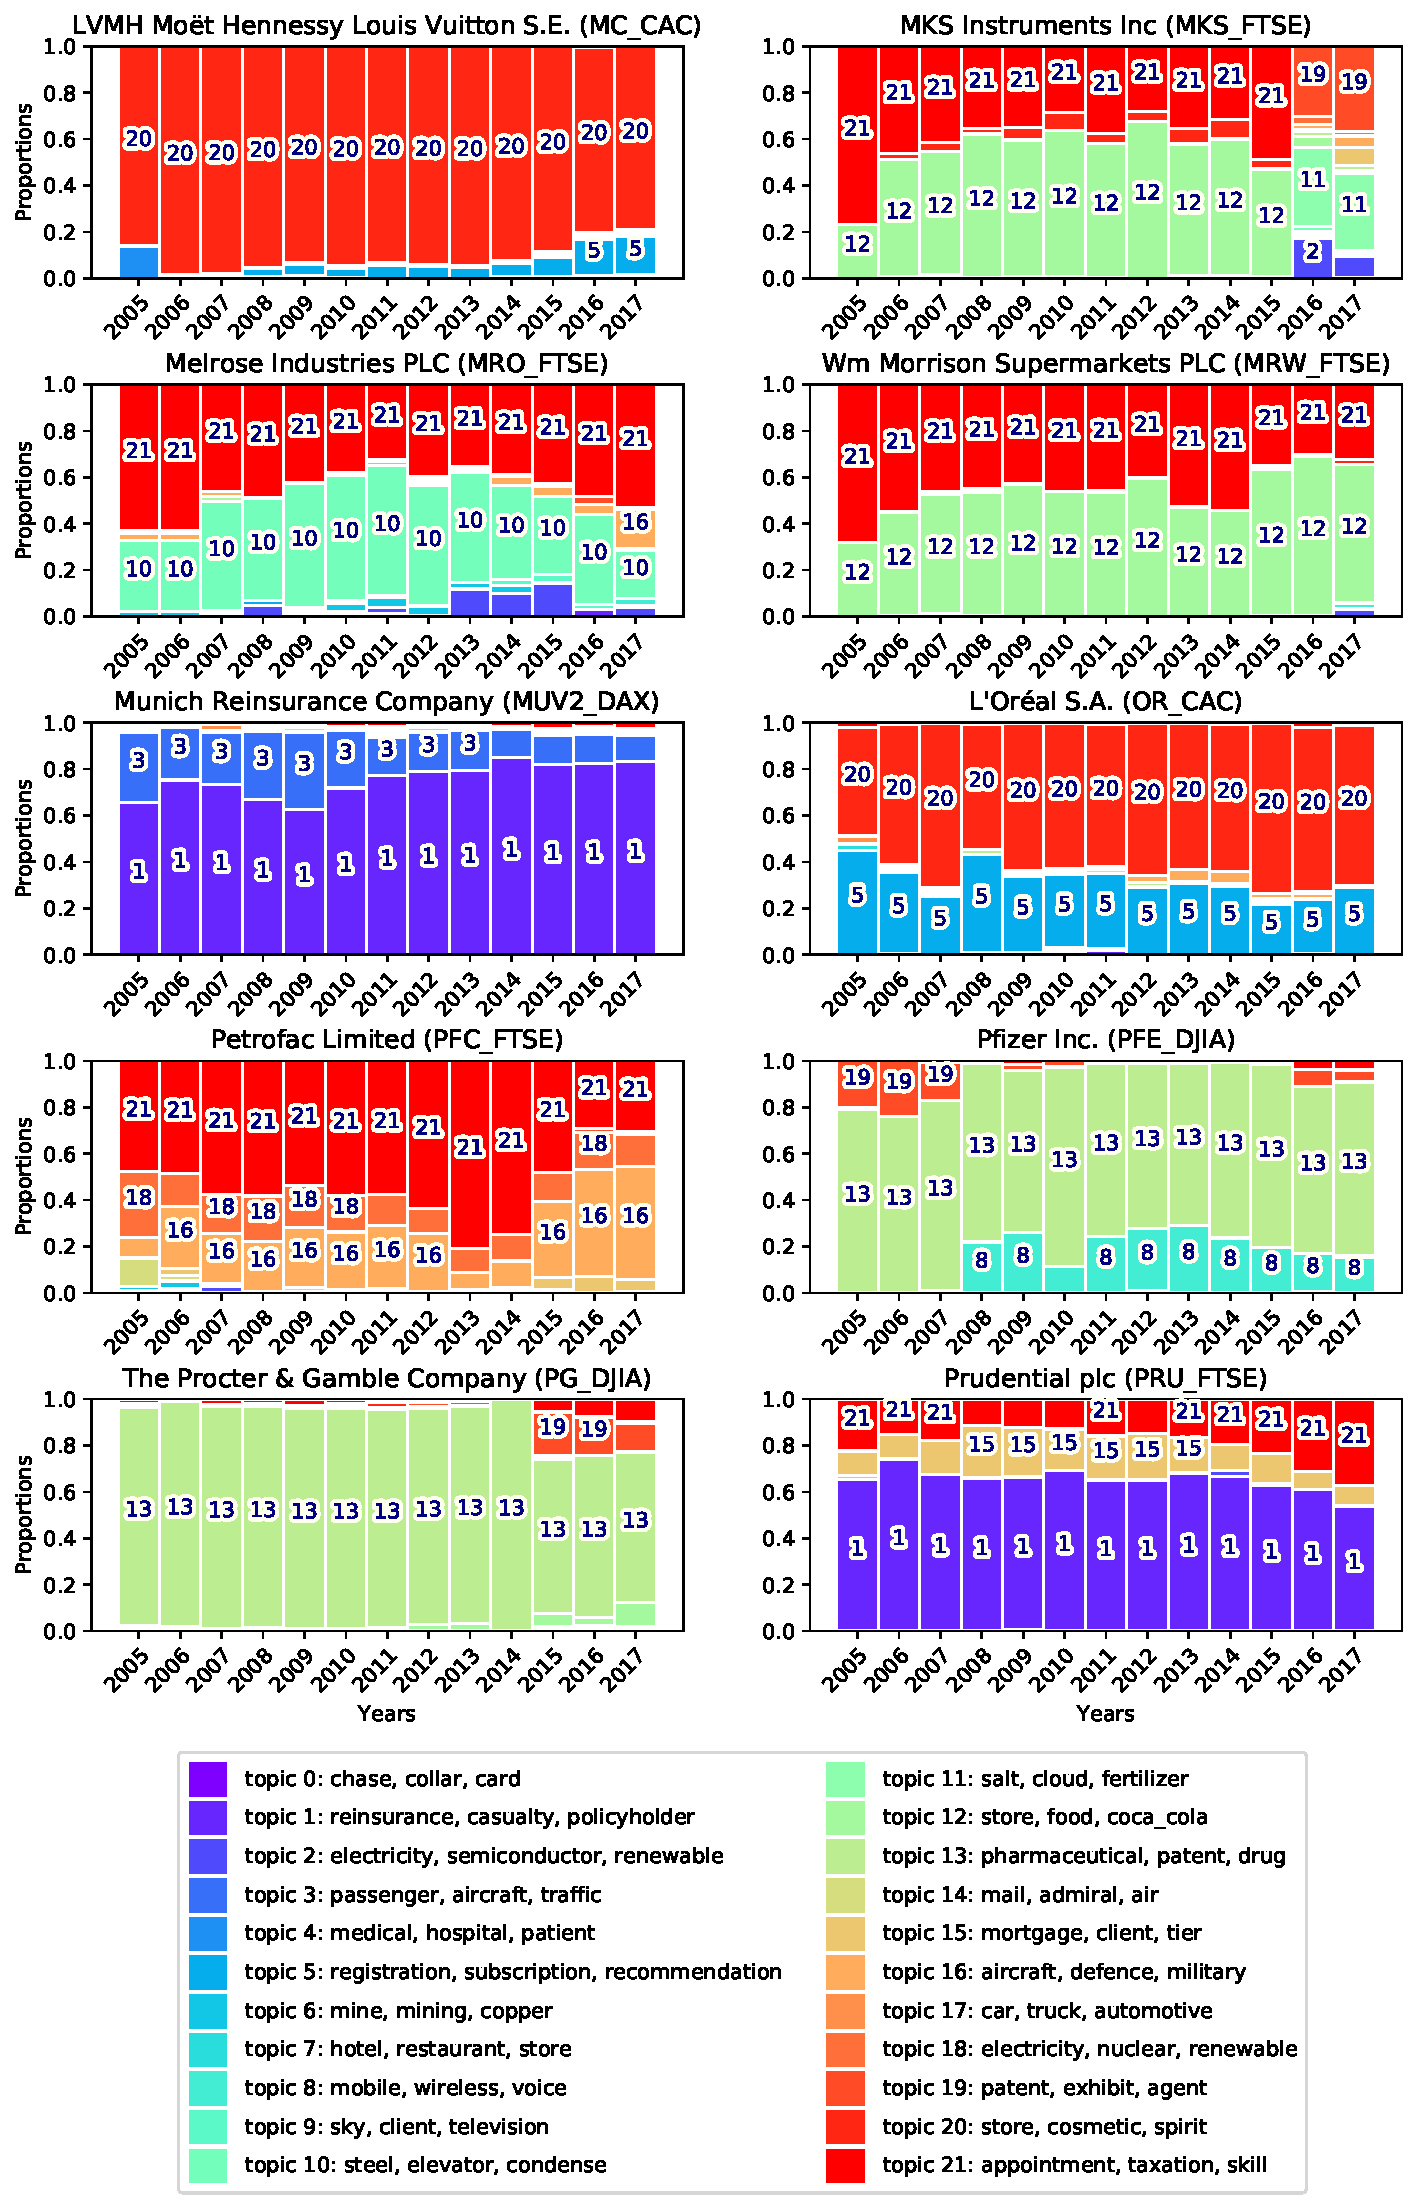
\includegraphics[width=0.85\linewidth]{images/companies_on_page_4.pdf}
\end{center}

\section{Topic distribution for target companies}
\begin{center}
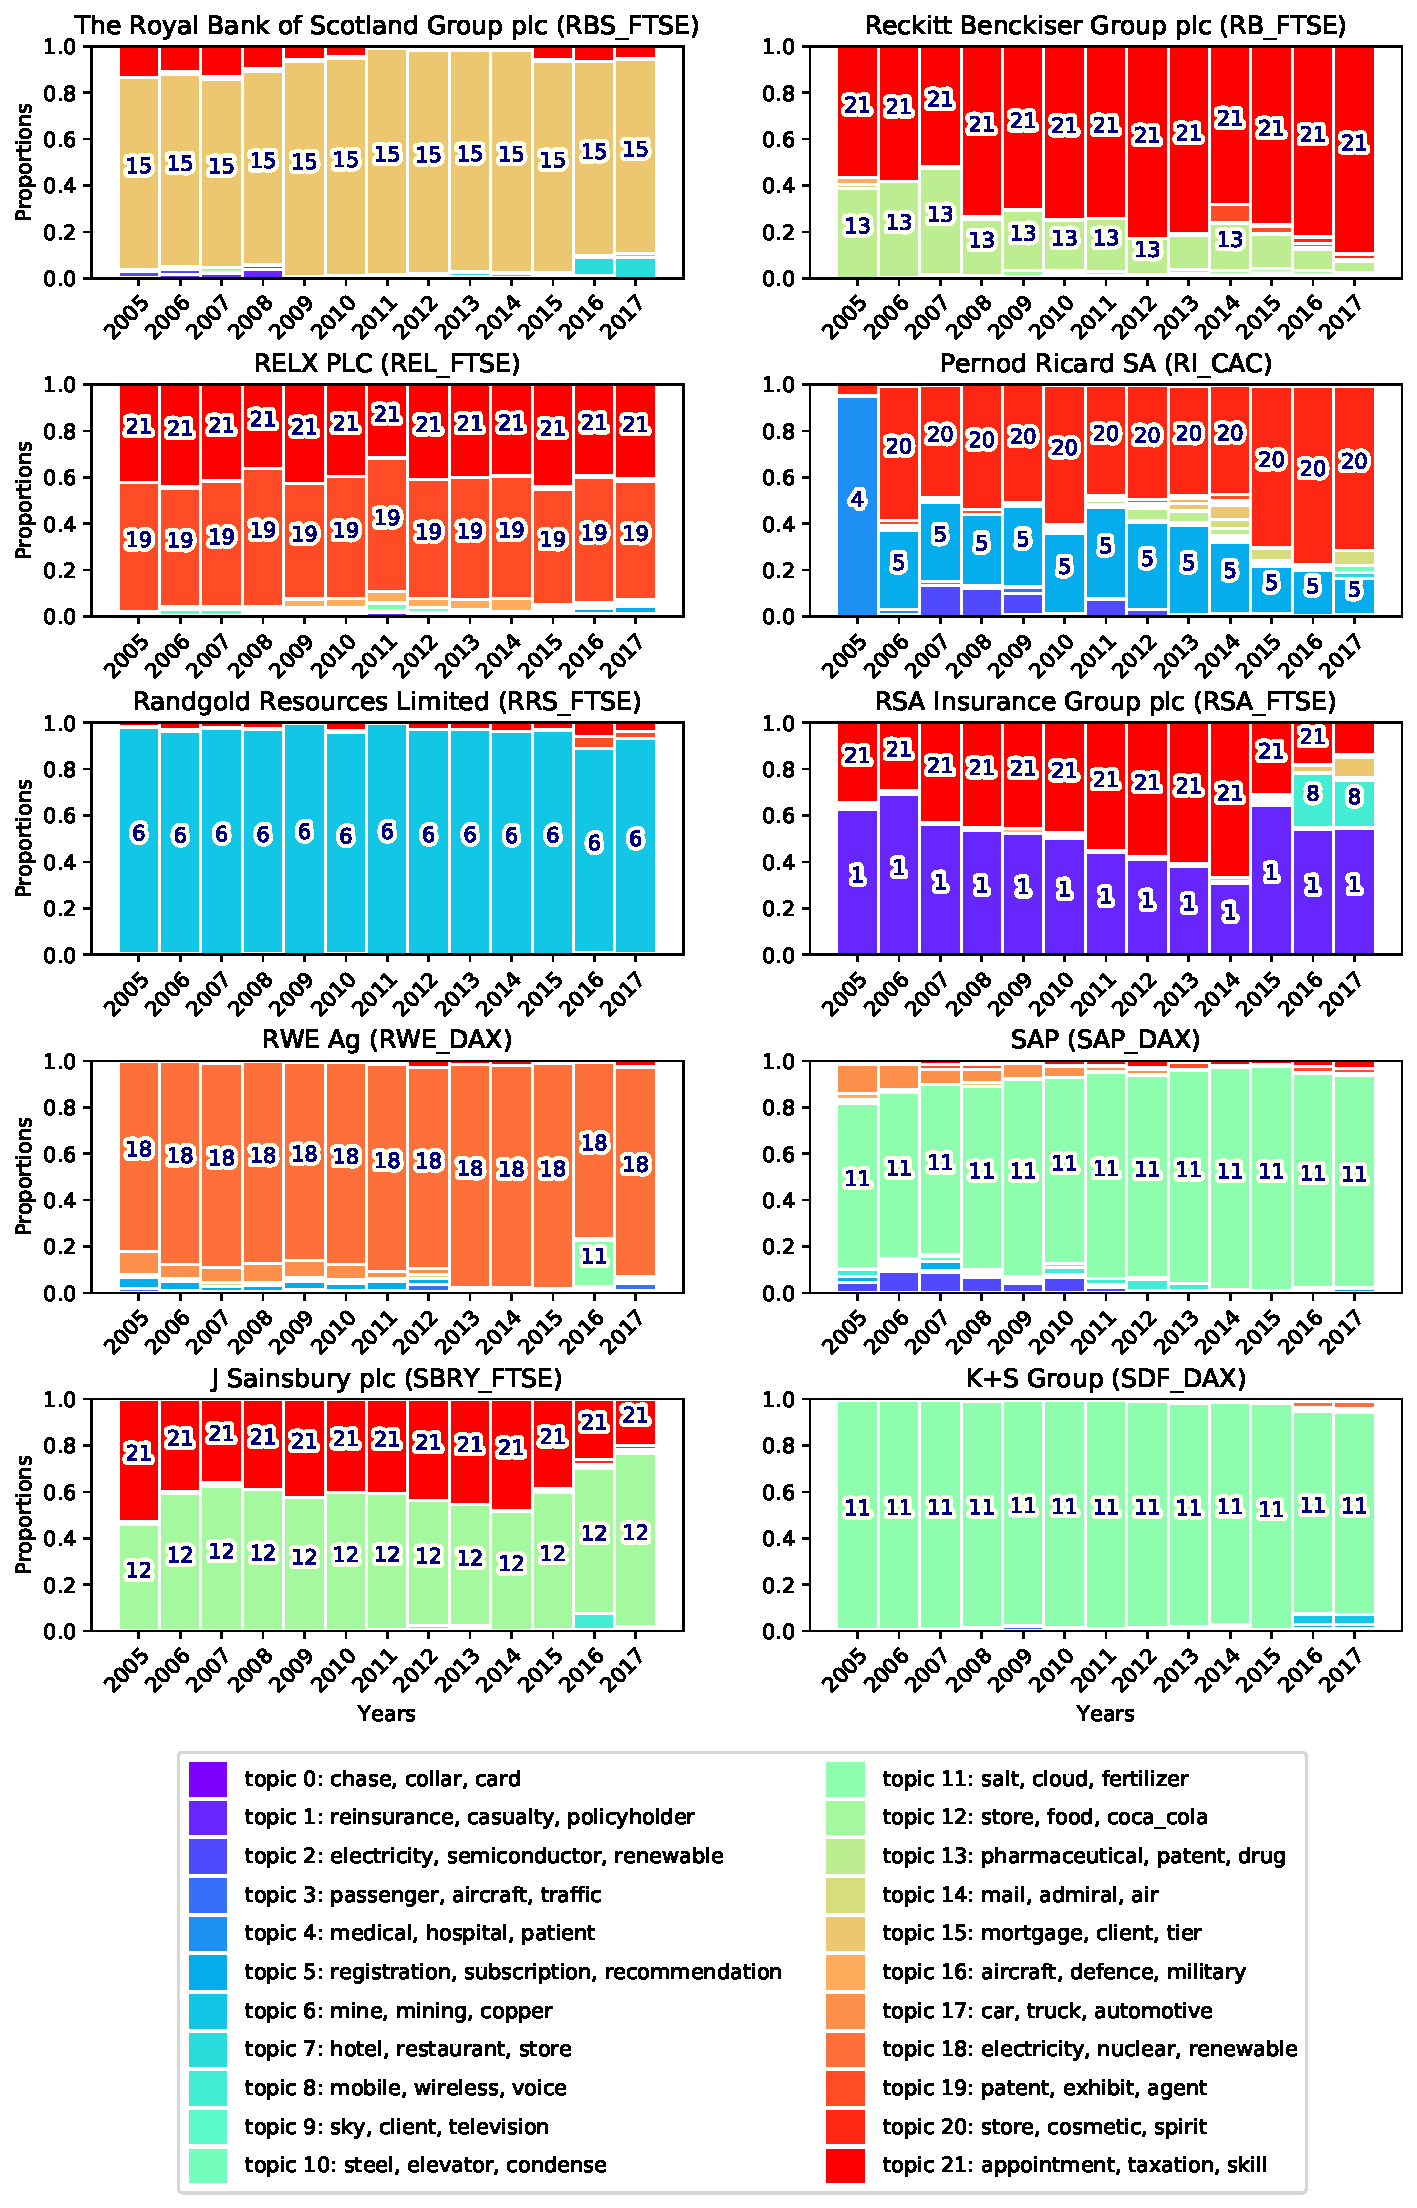
\includegraphics[width=0.85\linewidth]{images/companies_on_page_5.pdf}
\end{center}

\section{Topic distribution for target companies}
\begin{center}
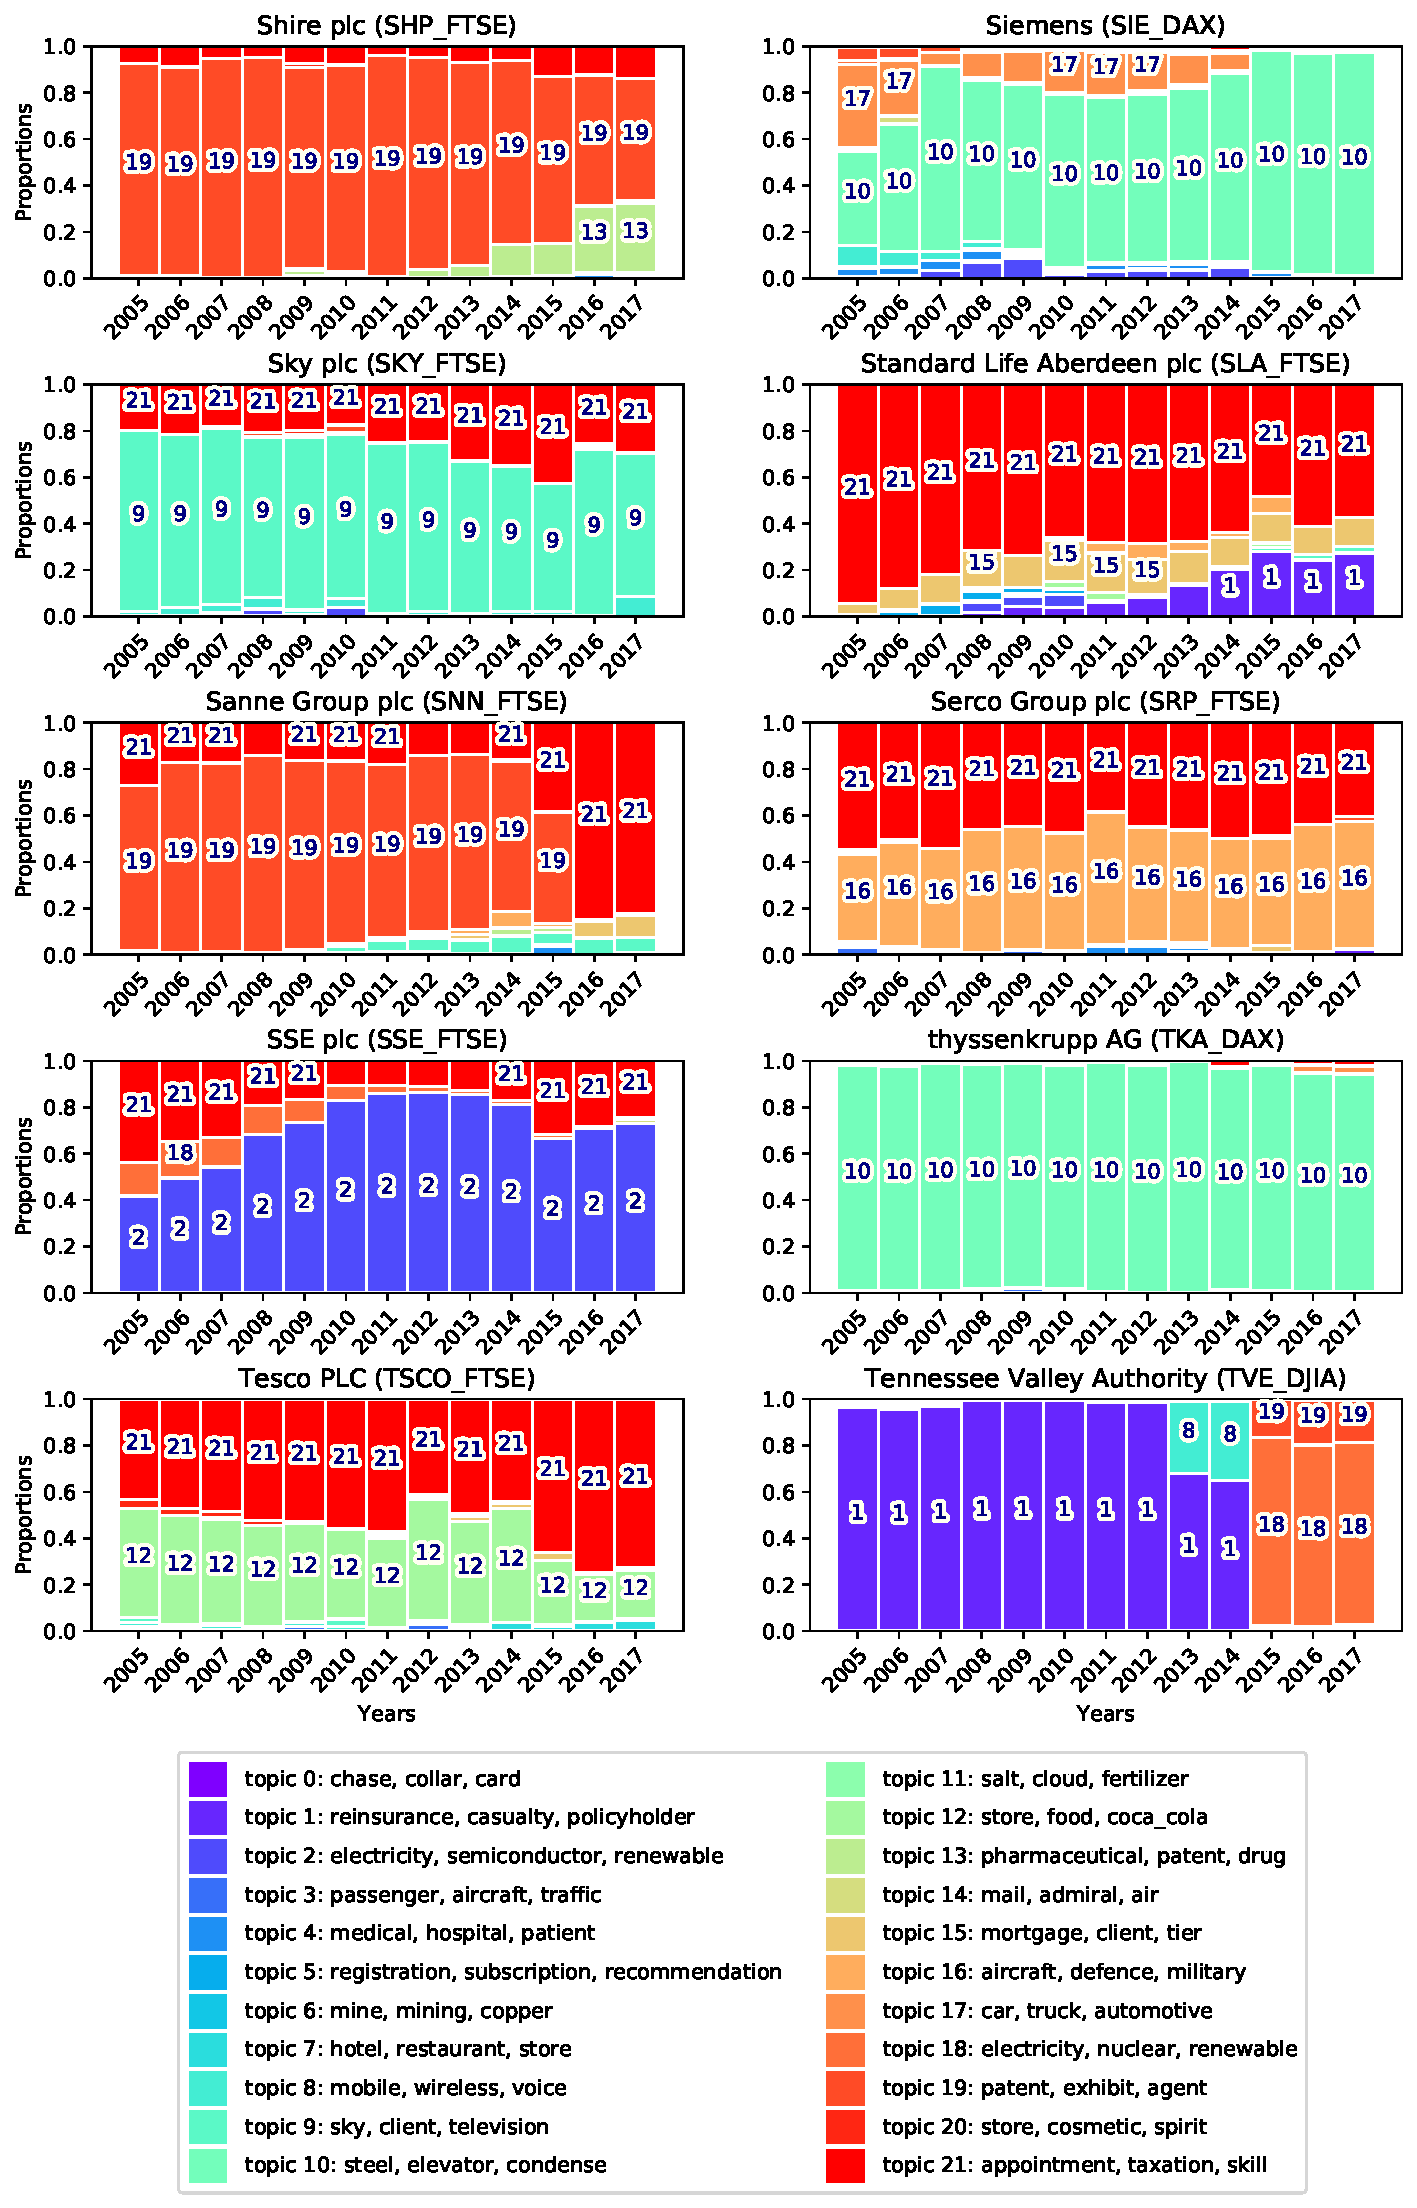
\includegraphics[width=0.85\linewidth]{images/companies_on_page_6.pdf}
\end{center}

\section{Topic distribution for target companies}
\begin{center}
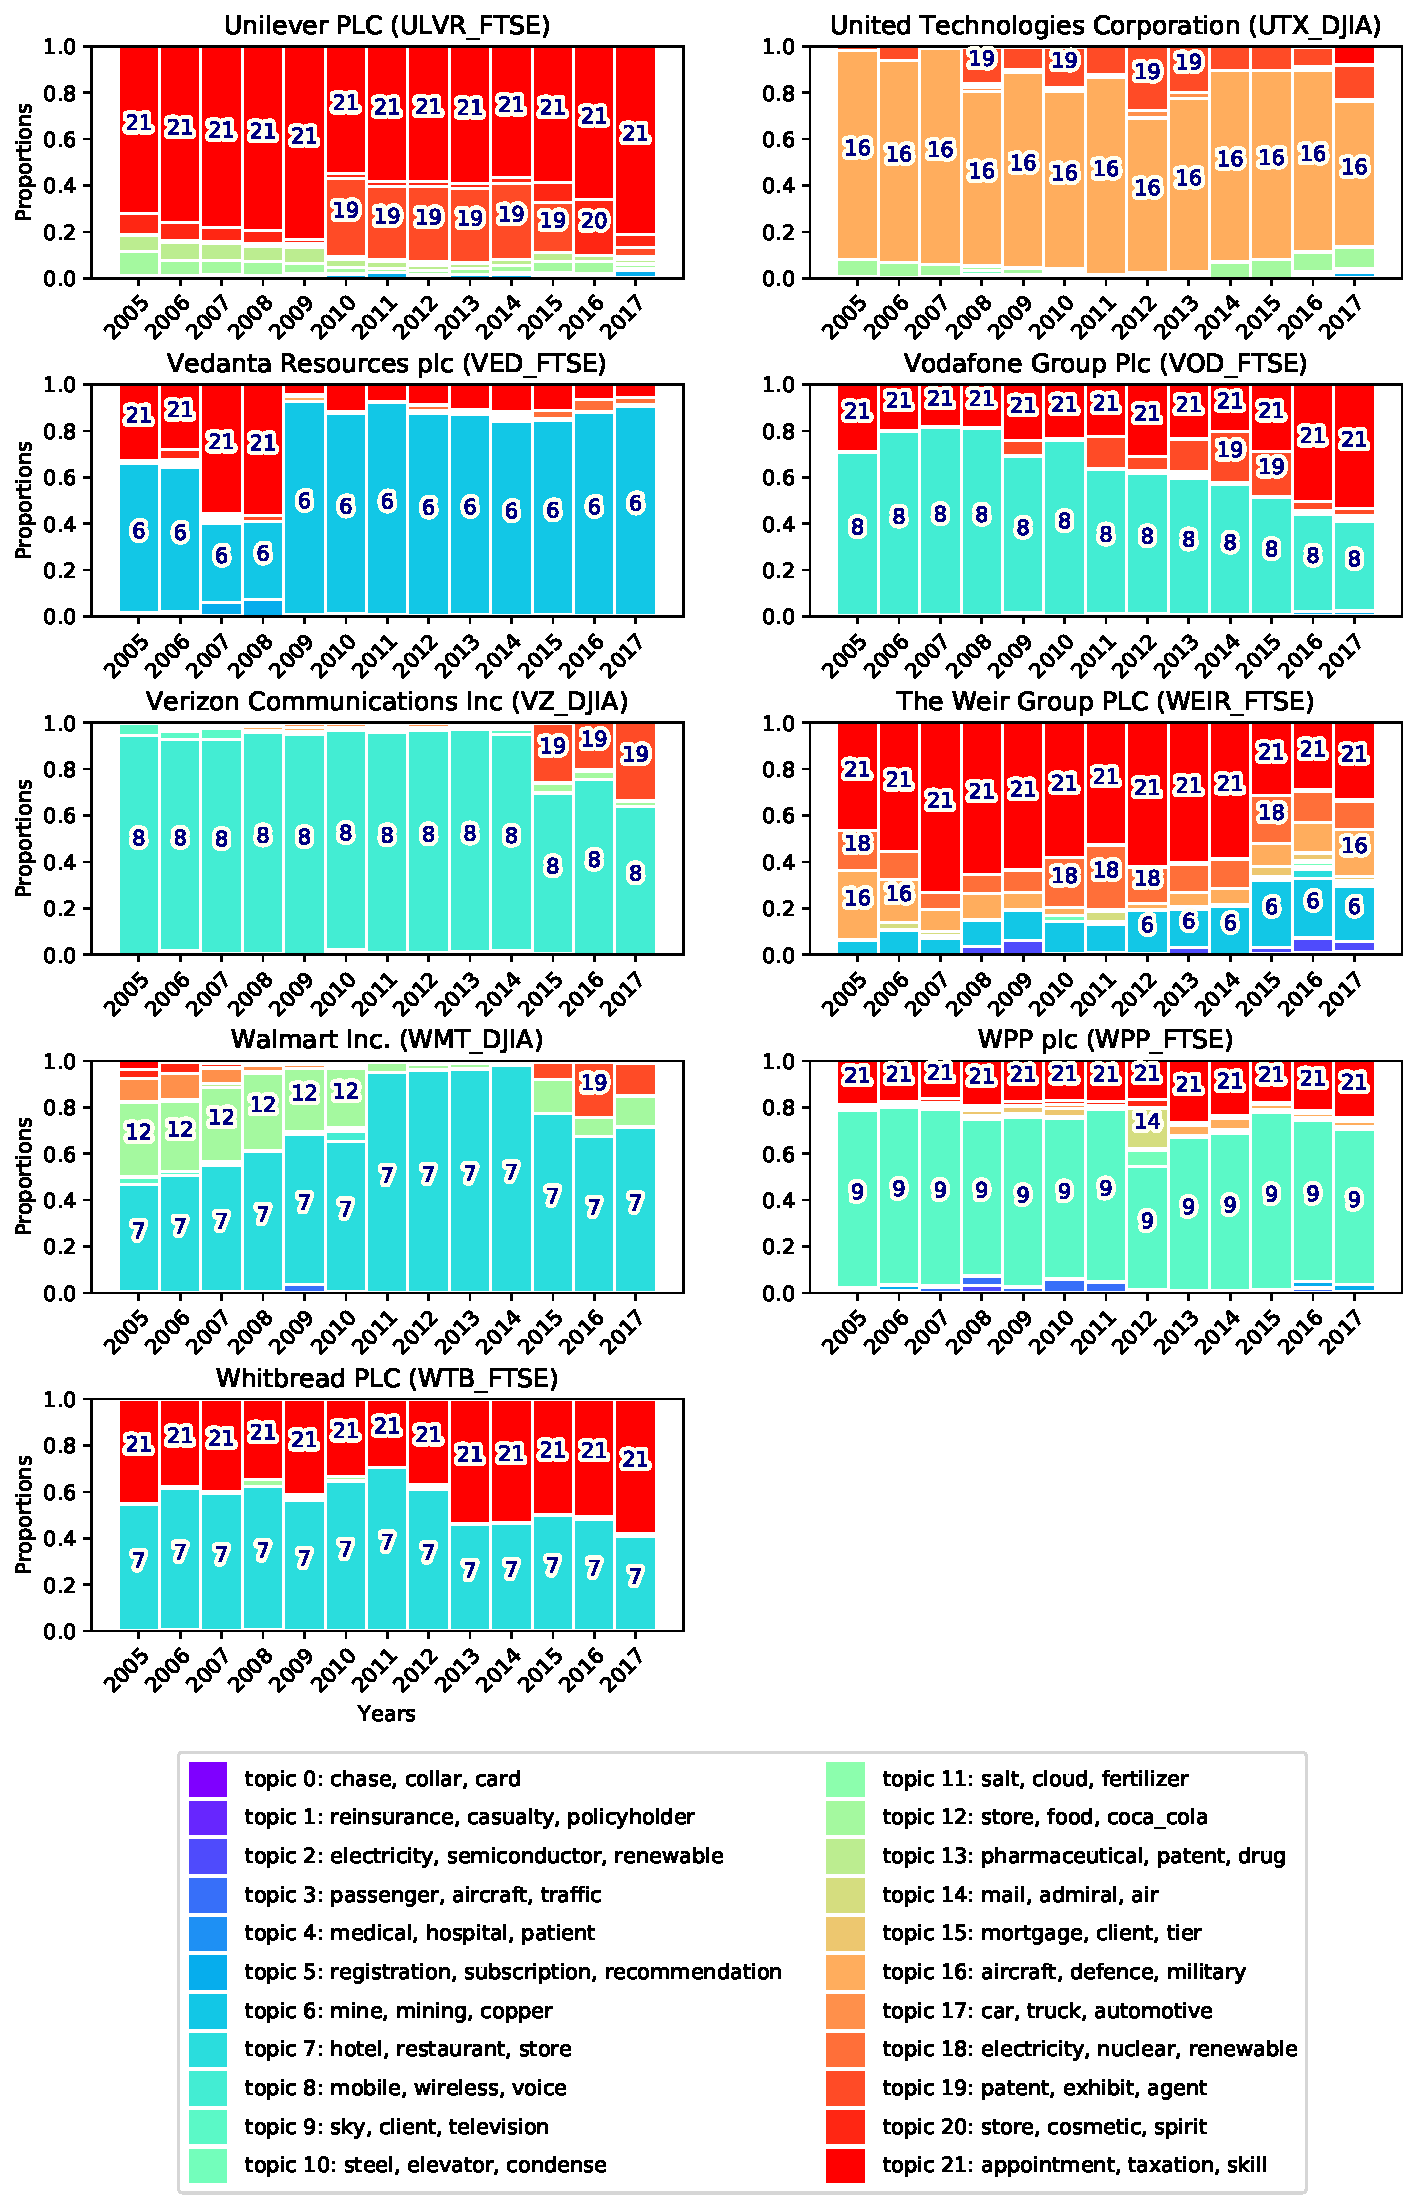
\includegraphics[width=0.85\linewidth]{images/companies_on_page_7.pdf}
\end{center}

\section{Shift of top five words over thirteen years}
\begin{center}
    \resizebox{\textwidth}{!}{
        \begin{tabular}{c|c|c|c|c|c|c|c|c|c|c|c|c|c}
        \hline
        \textbf{Topic Id} & \textbf{2005} & \textbf{2006} & \textbf{2007} & \textbf{2008} & \textbf{2009} & \textbf{2010} & \textbf{2011} & \textbf{2012} & \textbf{2013} & \textbf{2014} & \textbf{2015} & \textbf{2016} & \textbf{2017} \\ 
        \hline
        0 & chase & chase & chase & chase & chase & chase & chase & chase & collar & collar & collar & collar & collar \\ 
         & card & card & card & card & card & card & mortgage & fed & fed & fed & fed & equitable & equitable \\ 
         & heritage & heritage & mortgage & mortgage & mortgage & mortgage & card & collar & equitable & equitable & equitable & fed & ice \\ 
         & mortgage & mortgage & heritage & mutual & mutual & mutual & mutual & mortgage & chase & mortgage & accretion & accretion & accretion \\ 
         & news & news & news & news & stockholder & collar & fed & equitable & mortgage & accretion & unrealized & ice & fed \\ 
        \hline
        1 & reinsurance & reinsurance & reinsurance & reinsurance & reinsurance & reinsurance & reinsurance & reinsurance & reinsurance & reinsurance & reinsurance & reinsurance & reinsurance \\ 
         & casualty & casualty & casualty & casualty & casualty & casualty & casualty & casualty & casualty & casualty & casualty & solvency & solvency \\ 
         & policyholder & policyholder & policyholder & policyholder & policyholder & policyholder & policyholder & policyholder & policyholder & policyholder & policyholder & annuity & annuity \\ 
         & insurer & underwriting & underwriting & underwriting & annuity & annuity & catastrophe & subtotal & subtotal & annuity & solvency & policyholder & policyholder \\ 
         & underwriting & insurer & insurer & insurer & underwriting & underwriting & subtotal & underwriting & annuity & solvency & annuity & casualty & casualty \\ 
        \hline
        2 & memory & memory & condensed & electricity & electricity & electricity & electricity & electricity & electricity & electricity & electricity & electricity & electricity \\ 
         & dram & condensed & electricity & condensed & condensed & renewable & renewable & renewable & renewable & semiconductor & semiconductor & semiconductor & semiconductor \\ 
         & district & dram & semiconductor & semiconductor & semiconductor & station & station & transmission & transmission & transmission & rectifier & hybrid & hybrid \\ 
         & condensed & semiconductor & dram & chip & chip & semiconductor & storage & storage & storage & renewable & transmission & renewable & renewable \\ 
         & semiconductor & electricity & chip & dram & station & chip & semiconductor & station & semiconductor & storage & renewable & transmission & wholesale \\ 
        \hline
        3 & passenger & passenger & passenger & passenger & crisis & crisis & passenger & passenger & passenger & passenger & passenger & passenger & air \\ 
         & aircraft & aircraft & aircraft & aircraft & passenger & passenger & crisis & aircraft & aircraft & aircraft & aircraft & air & passenger \\ 
         & traffic & traffic & cargo & crisis & aircraft & traffic & traffic & traffic & traffic & flight & air & aircraft & aircraft \\ 
         & air & air & traffic & traffic & traffic & aircraft & aircraft & crisis & flight & cargo & flight & parameter & parameter \\ 
         & cargo & cargo & air & cargo & cargo & cargo & flight & flight & cargo & traffic & cargo & flight & cargo \\ 
        \hline
        4 & medical & medical & medical & medical & medical & medical & medical & medical & medical & medical & medical & medical & medical \\ 
         & preference & preference & preference & patient & patient & hospital & hospital & hospital & hospital & hospital & hospital & hospital & hospital \\ 
         & patient & patient & patient & hospital & hospital & patient & patient & patient & patient & patient & patient & patient & patient \\ 
         & hospital & hospital & hospital & preference & preference & dialysis & dialysis & dialysis & dialysis & dialysis & glance & dialysis & thousand \\ 
         & dialysis & dialysis & dialysis & dialysis & dialysis & preference & glance & glance & glance & glance & dialysis & glance & dialysis \\ 
        \hline
        5 & registration & registration & registration & registration & registration & registration & registration & registration & registration & registration & registration & registration & registration \\ 
         & shelf & client & subscription & subscription & subscription & subscription & subscription & subscription & subscription & subscription & recommendation & recommendation & emission \\ 
         & client & subscription & client & client & extraordinary & preferred & appointment & appointment & recommendation & recommendation & subscription & emission & recommendation \\ 
         & affiliate & affiliate & affiliate & thousand & thousand & appointment & preferred & recommendation & appointment & appointment & emission & subscription & water \\ 
         & convertible & shelf & thousand & extraordinary & authorization & extraordinary & extraordinary & breakdown & deputy & deputy & appointment & water & subscription \\ 
        \hline
        6 & mine & mine & mine & mine & mine & mine & mine & mine & mine & mine & mine & mine & mine \\ 
         & gold & gold & copper & copper & copper & copper & copper & mining & mining & mining & mining & mining & mining \\ 
         & mining & copper & mining & mining & mining & mining & mining & copper & copper & gold & gold & gold & gold \\ 
         & ore & mining & gold & ore & ore & ore & ore & gold & gold & copper & copper & copper & ore \\ 
         & copper & ore & ore & gold & gold & mineral & gold & ore & ore & ore & ore & ore & copper \\ 
        \hline
        7 & hotel & hotel & hotel & hotel & hotel & hotel & hotel & hotel & hotel & hotel & hotel & restaurant & restaurant \\ 
         & restaurant & restaurant & restaurant & restaurant & restaurant & restaurant & restaurant & restaurant & restaurant & restaurant & restaurant & store & store \\ 
         & travel & travel & club & rent & store & store & store & store & store & store & store & hotel & hotel \\ 
         & club & club & rent & franchise & rent & rent & rent & rent & sam club & club & club & club & club \\ 
         & premier & room & travel & club & franchise & franchise & sam club & sam club & club & sam club & premier inn & commerce & roi \\ 
        \hline
        8 & mobile & mobile & mobile & mobile & mobile & mobile & mobile & mobile & mobile & mobile & mobile & mobile & mobile \\ 
         & wireless & wireless & wireless & wireless & wireless & wireless & wireless & wireless & wireless & wireless & wireless & wireless & wireless \\ 
         & voice & voice & voice & voice & voice & voice & voice & voice & spectrum & spectrum & spectrum & device & device \\ 
         & operator & operator & operator & operator & operator & operator & operator & spectrum & voice & voice & device & spectrum & spectrum \\ 
         & telecommunication & telecommunication & device & device & device & device & spectrum & operator & operator & speed & voice & license & license \\ 
        \hline
        9 & sky & sky & sky & sky & sky & sky & sky & sky & sky & sky & client & client & client \\ 
         & client & client & client & television & television & television & client & client & client & client & sky & sky & sky \\ 
         & television & television & television & client & client & client & television & television & television & television & digital & digital & digital \\ 
         & advertising & advertising & advertising & advertising & advertising & advertising & advertising & advertising & advertising & digital & headline & headline & headline \\ 
         & subscriber & digital & digital & digital & digital & digital & digital & resort & resort & headline & advertising & advertising & advertising \\ 
        \hline
        10 & steel & steel & steel & steel & steel & steel & steel & steel & steel & steel & steel & steel & steel \\ 
         & automotive & elevator & elevator & elevator & elevator & condense & condense & condense & condense & condense & elevator & elevator & elevator \\ 
         & elevator & automotive & automotive & stainless & stainless & elevator & elevator & elevator & elevator & elevator & condense & therein & therein \\ 
         & stainless & stainless & stainless & automotive & condense & stainless & stainless & stainless & intake & intake & intake & intake & severance \\ 
         & raw & raw & engineering & intake & intake & intake & intake & intake & stainless & therein & therein & severance & renewable \\ 
        \hline
        11 & salt & salt & salt & salt & salt & salt & salt & salt & salt & cloud & cloud & cloud & cloud \\ 
         & fertilizer & fertilizer & fertilizer & fertilizer & fertilizer & fertilizer & potash & cloud & cloud & salt & salt & subscription & subscription \\ 
         & thousand & potash magnesium & potash magnesium & potash magnesium & potash magnesium & potash & potash magnesium & potash & subscription & subscription & subscription & salt & salt \\ 
         & potash magnesium & waste & potash & potash & potash & potash magnesium & fertilizer & potash magnesium & potash magnesium & potash magnesium & license & license & license \\ 
         & waste & thousand & waste & object & object & object & cloud & subscription & potash & license & organization & organization & digital \\ 
        \hline
        12 & store & store & store & store & store & store & store & store & store & store & store & store & store \\ 
         & food & food & food & food & food & food & food & food & food & bottle & bottle & exhibit & bottle \\ 
         & coca cola & coca cola & coca cola & coca cola & coca cola & coca cola & coca cola & coca cola & bottle & food & coca cola & bottle & exhibit \\ 
         & home depot & home depot & bottle & bottle & bottle & bottle & bottle & bottle & coca cola & coca cola & exhibit & coca cola & coca cola \\ 
         & bottle & bottle & home depot & beverage & beverage & beverage & space & space & beverage & exhibit & food & food & registrant \\ 
        \hline
        13 & pharmaceutical & pharmaceutical & pharmaceutical & pharmaceutical & pharmaceutical & pharmaceutical & pharmaceutical & pharmaceutical & pharmaceutical & pharmaceutical & pharmaceutical & patent & patent \\ 
         & stockholder & stockholder & patent & patent & patent & patent & patent & patent & patent & patent & patent & pharmaceutical & pharmaceutical \\ 
         & patent & patent & stockholder & stockholder & adhesive & adhesive & adhesive & drug & drug & patient & patient & patient & patient \\ 
         & behind & behind & behind & adhesive & drug & drug & drug & adhesive & adhesive & drug & drug & drug & drug \\ 
         & raw & raw & laundry & laundry & laundry & divestiture & divestiture & patient & patient & adhesive & gamble & gamble & legacy \\ 
        \hline
        14 & mail & mail & mail & mail & mail & mail & mail & mail & admiral & admiral & admiral & admiral & admiral \\ 
         & noncurrent & logistic & air & air & air & air & admiral & admiral & mail & air & parcel & inde & inde \\ 
         & logistic & noncurrent & logistic & engineering & engineering & engineering & air & air & air & mail & car & parcel & parcel \\ 
         & air & air & engineering & logistic & admiral & admiral & engineering & engineering & engineering & car & engineering & engineering & engineering \\ 
         & engineering & engineering & noncurrent & admiral & logistic & hydrogen & hydrogen & car & car & engineering & air & car & car \\ 
        \hline
        15 & mortgage & mortgage & mortgage & mortgage & mortgage & mortgage & mortgage & mortgage & mortgage & mortgage & client & client & client \\ 
         & client & client & client & client & client & client & client & client & client & client & mortgage & mortgage & mortgage \\ 
         & card & card & card & card & tier & tier & tier & tier & tier & tier & tier & tier & tier \\ 
         & branch & branch & branch & tier & card & preference & wholesale & stress & stress & stress & stress & stress & stress \\ 
         & tier & tier & tier & wholesale & wholesale & wholesale & preference & wholesale & wealth & wealth & wealth & branch & load \\ 
        \hline
        16 & aircraft & aircraft & aircraft & aircraft & aircraft & aircraft & aircraft & aircraft & aircraft & aircraft & aircraft & defence & defence \\ 
         & defence & defence & defence & defence & defence & defence & defence & defence & defence & defence & defence & aircraft & air \\ 
         & military & military & military & military & military & military & military & military & military & condensed & air & air & aircraft \\ 
         & space & air & air & air & air & air & air & condense & condensed & condense & condense & engineering & engineering \\ 
         & air & space & condense & carrier & carrier & condense & condense & condensed & condense & military & engineering & condense & engine \\ 
        \hline
        17 & car & car & car & car & car & car & car & car & car & car & car & car & car \\ 
         & truck & truck & truck & truck & truck & truck & truck & automotive & automotive & automotive & automotive & truck & truck \\ 
         & automobile & automobile & automobile & bus & crisis & crisis & automotive & truck & truck & truck & truck & automotive & automotive \\ 
         & engine & bus & bus & automobile & bus & emission & emission & emission & emission & bus & bus & bus & bus \\ 
         & marketable & engine & emission & emission & emission & bus & bus & bus & bus & emission & emission & emission & mobility \\ 
        \hline
        18 & electricity & electricity & electricity & electricity & electricity & electricity & electricity & electricity & electricity & electricity & nuclear & nuclear & nuclear \\ 
         & water & water & nuclear & nuclear & nuclear & nuclear & nuclear & nuclear & nuclear & nuclear & electricity & electricity & electricity \\ 
         & nuclear & nuclear & water & water & emission & renewable & renewable & renewable & renewable & renewable & renewable & coal & coal \\ 
         & emission & emission & emission & emission & coal & emission & coal & coal & coal & coal & coal & renewable & renewable \\ 
         & coal & coal & coal & coal & renewable & coal & emission & emission & emission & emission & emission & fire & fire \\ 
        \hline
        19 & patent & patent & patent & patent & patent & patent & agent & agent & agent & agent & agent & exhibit & exhibit \\ 
         & pharmaceutical & pharmaceutical & pharmaceutical & pharmaceutical & pharmaceutical & exhibit & lender & lender & lender & lender & exhibit & registrant & registrant \\ 
         & medical & medical & medical & medical & medical & pharmaceutical & exhibit & exhibit & exhibit & trustee & registrant & proxy & proxy \\ 
         & patient & patient & patient & patient & patient & agent & patent & patent & issuer & exhibit & trustee & paragraph & paragraph \\ 
         & drug & drug & taxation & taxation & exhibit & patient & pharmaceutical & license & registrant & issuer & lender & forth & forth \\ 
        \hline
        20 & cosmetic & store & store & store & store & store & store & store & store & store & store & beauty & beauty \\ 
         & store & cosmetic & cosmetic & cosmetic & spirit & spirit & spirit & spirit & cosmetic & cosmetic & vision & vision & digital \\ 
         & spirit & spirit & spirit & spirit & cosmetic & cosmetic & cosmetic & cosmetic & wine & vision & cosmetic & cosmetic & cosmetic \\ 
         & woman & luxury & luxury & luxury & wine & wine & wine & wine & spirit & optical & beauty & store & vision \\ 
         & luxury & woman & campaign & campaign & luxury & campaign & campaign & selective & beauty & beauty & optical & digital & store \\ 
        \hline
        21 & taxation & taxation & taxation & taxation & appointment & appointment & appointment & appointment & appointment & appointment & appointment & appointment & appointment \\ 
         & turnover & appointment & appointment & appointment & taxation & taxation & taxation & taxation & skill & skill & skill & colleague & colleague \\ 
         & appointment & preference & preference & preference & preference & pence & attend & skill & taxation & colleague & colleague & skill & skill \\ 
         & preference & turnover & undertaking & pence & pence & attend & skill & attend & attend & taxation & diversity & diversity & culture \\ 
         & undertaking & undertaking & pence & undertaking & attend & nomination & pence & nomination & colleague & attend & taxation & stakeholder & diversity \\ 
    \end{tabular}}
\end{center}

\section{Returns on individual topics during experiment time frame}
\begin{center}
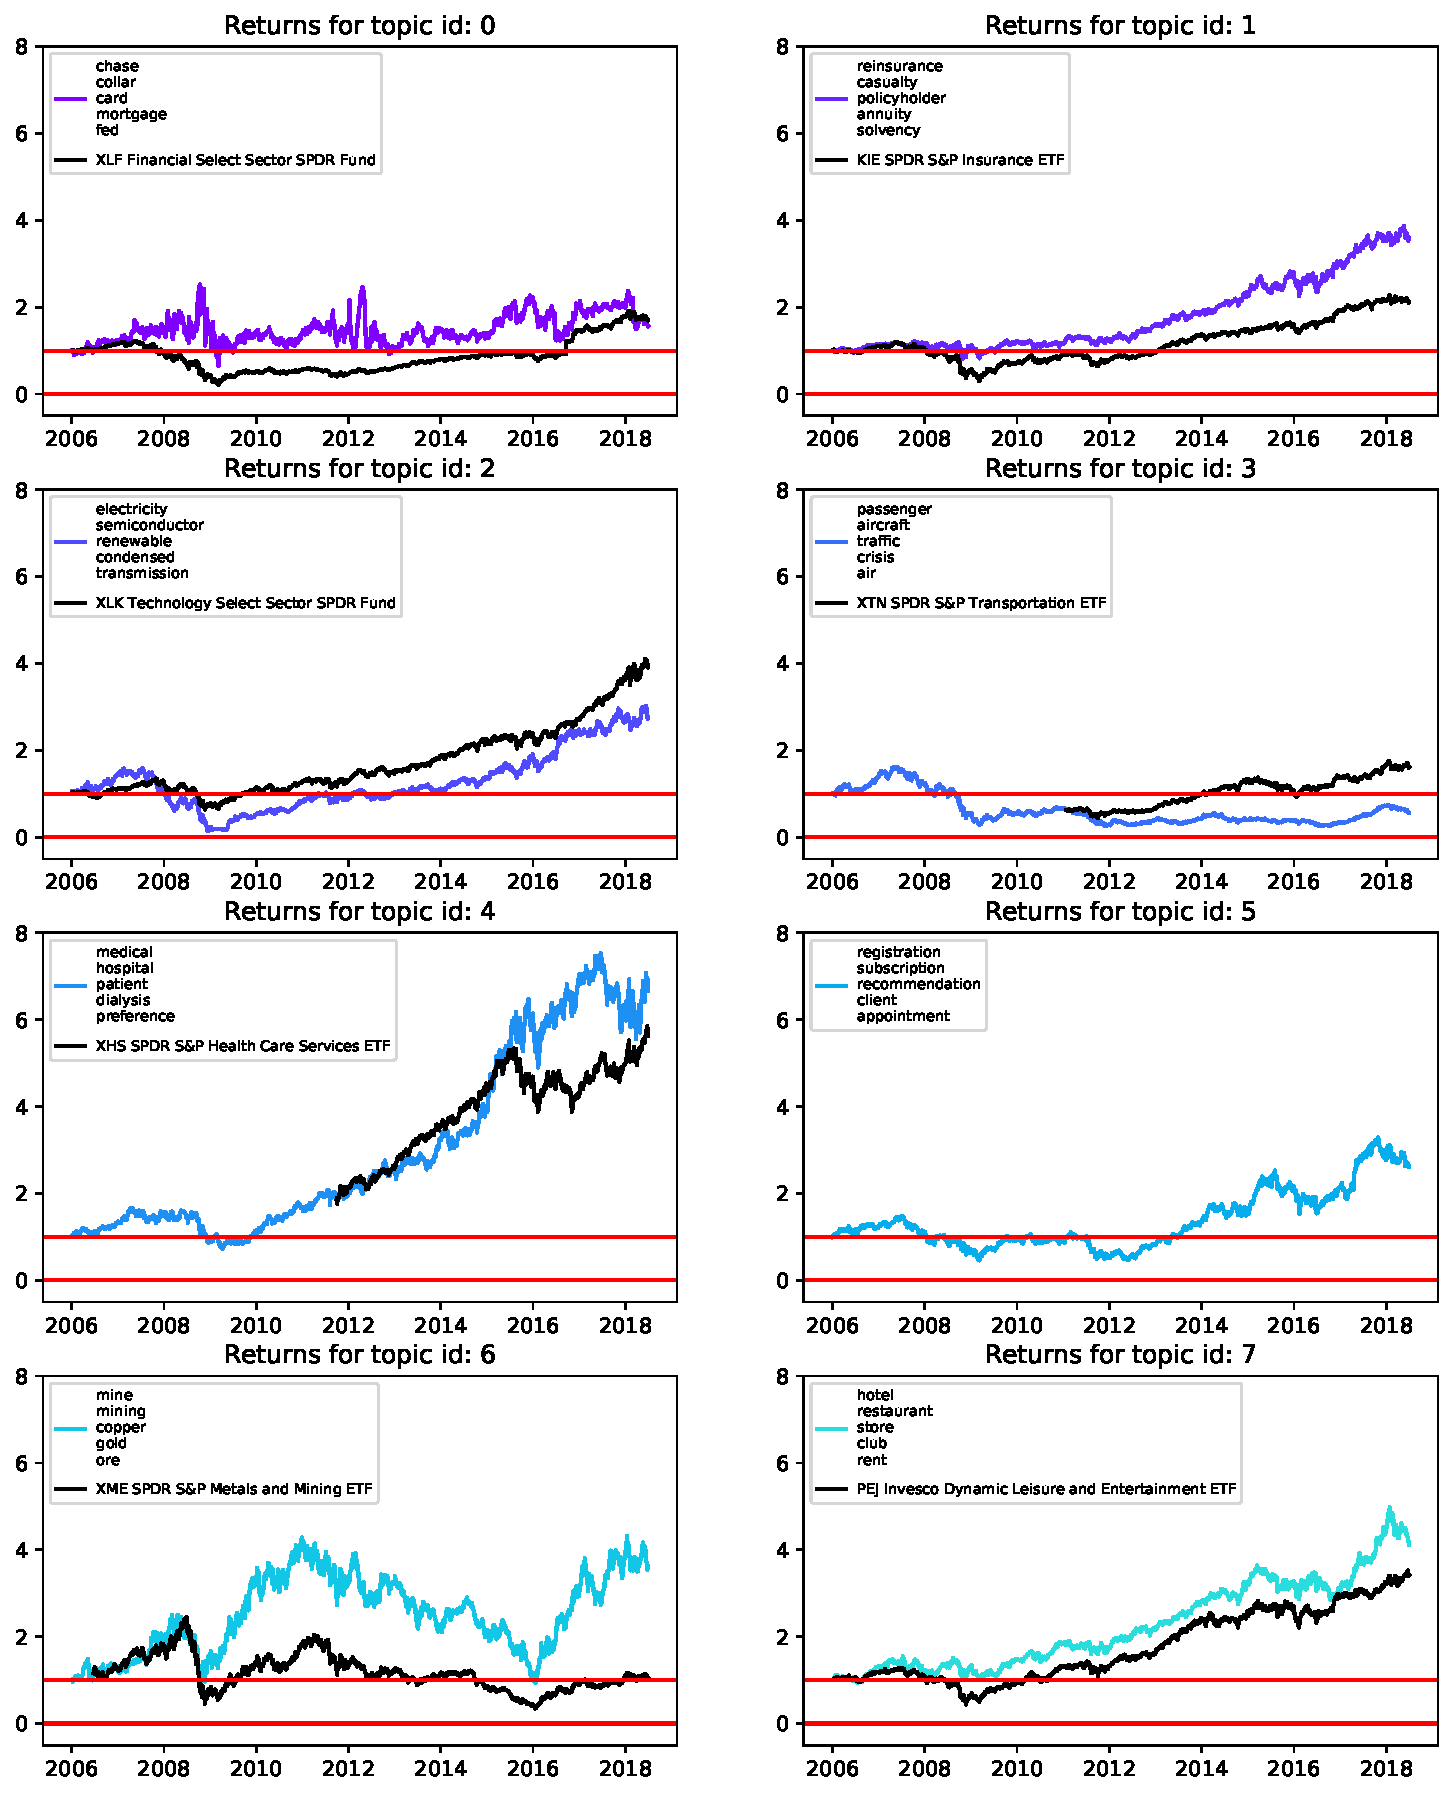
\includegraphics[width=1\linewidth]{images/returns_per_topic_page_0.pdf}
\end{center}

\section{Returns on individual topics during experiment time frame}
\begin{center}
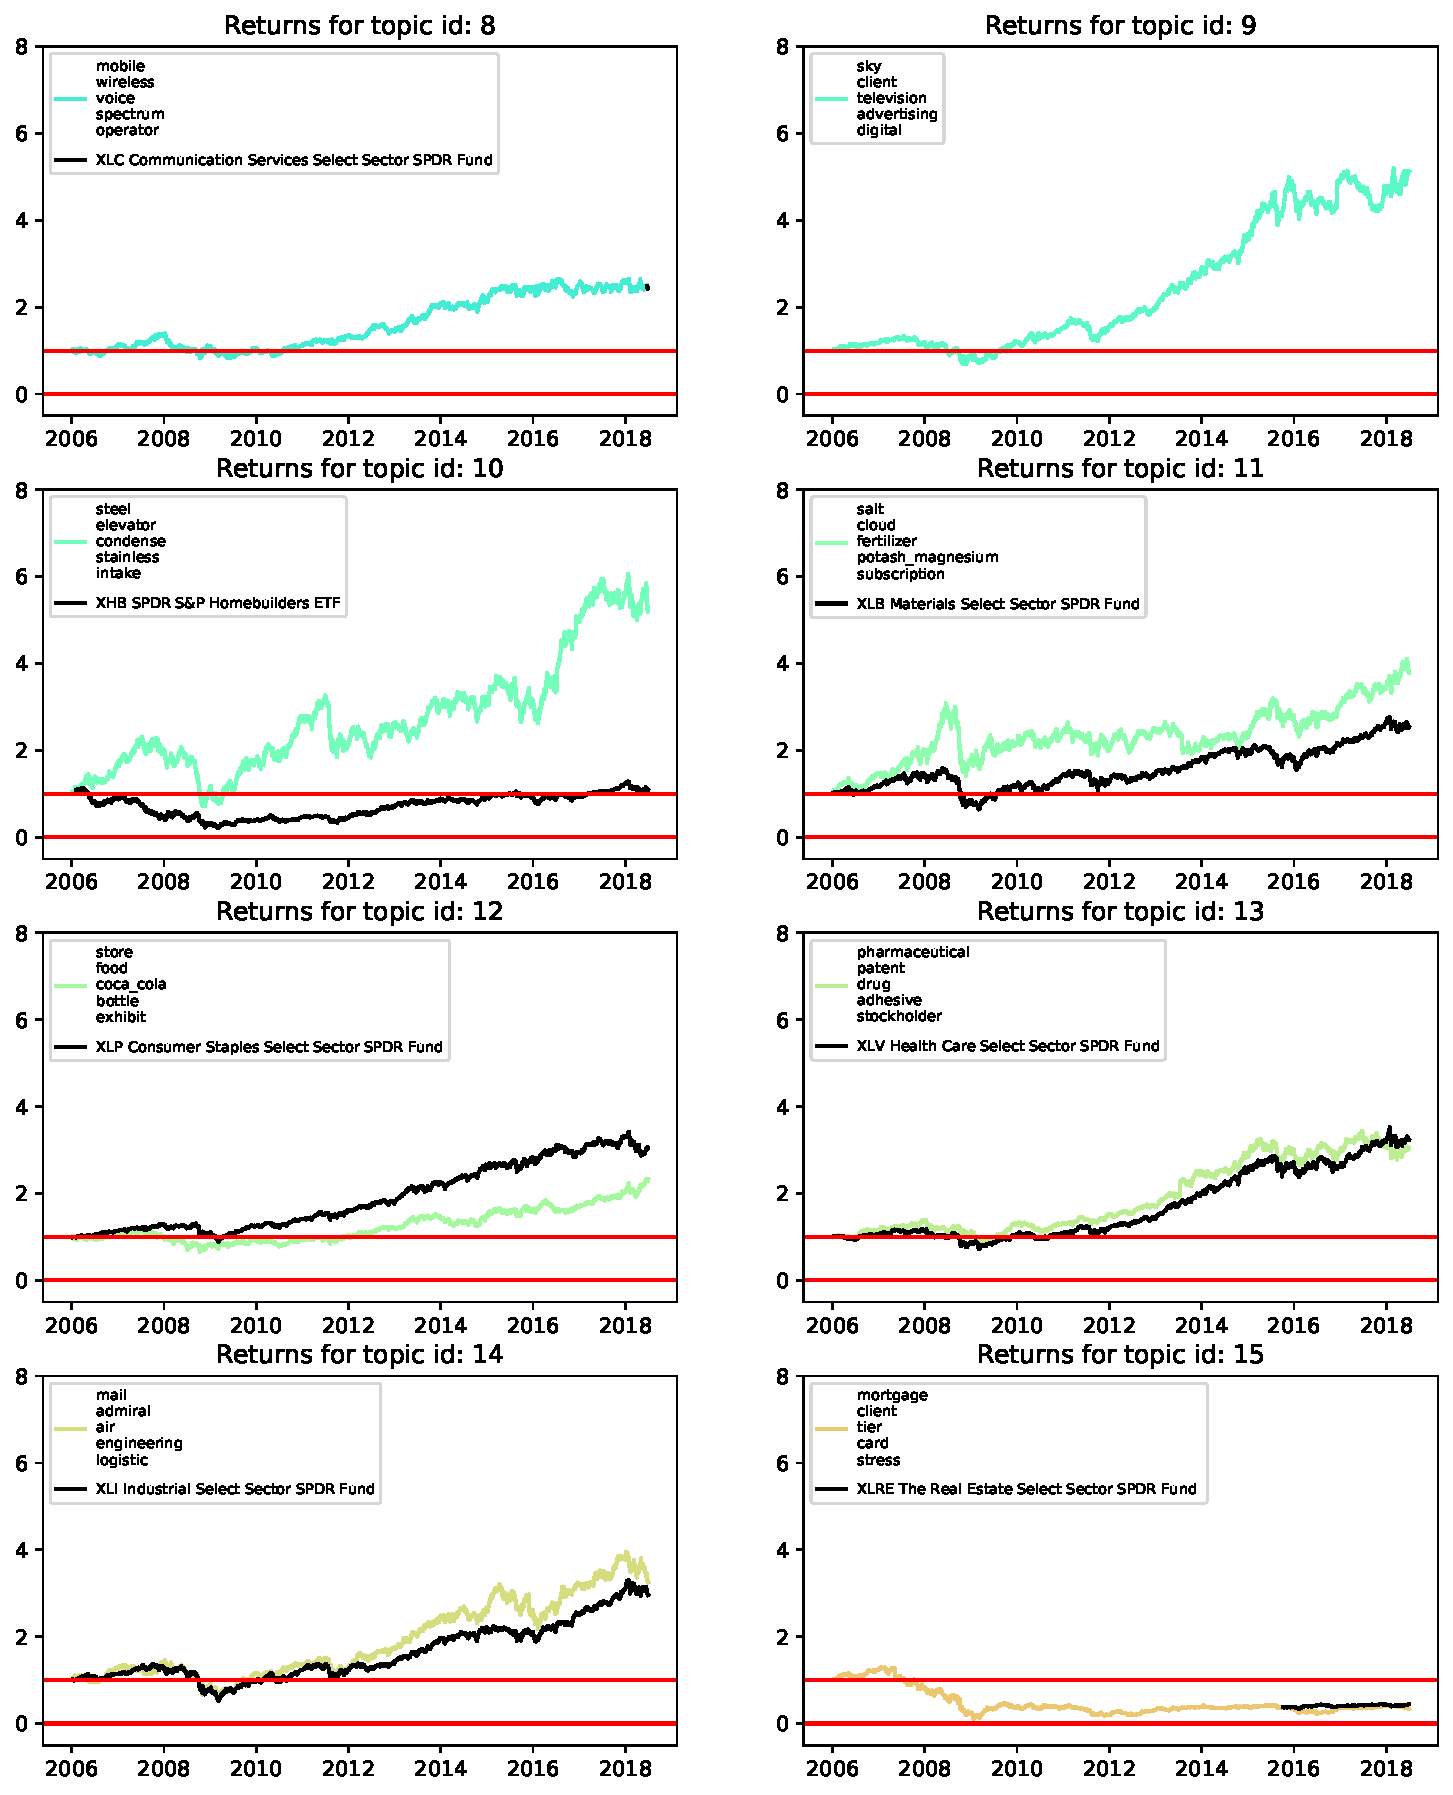
\includegraphics[width=1\linewidth]{images/returns_per_topic_page_1.pdf}
\end{center}

\section{Returns on individual topics during experiment time frame}
\begin{center}
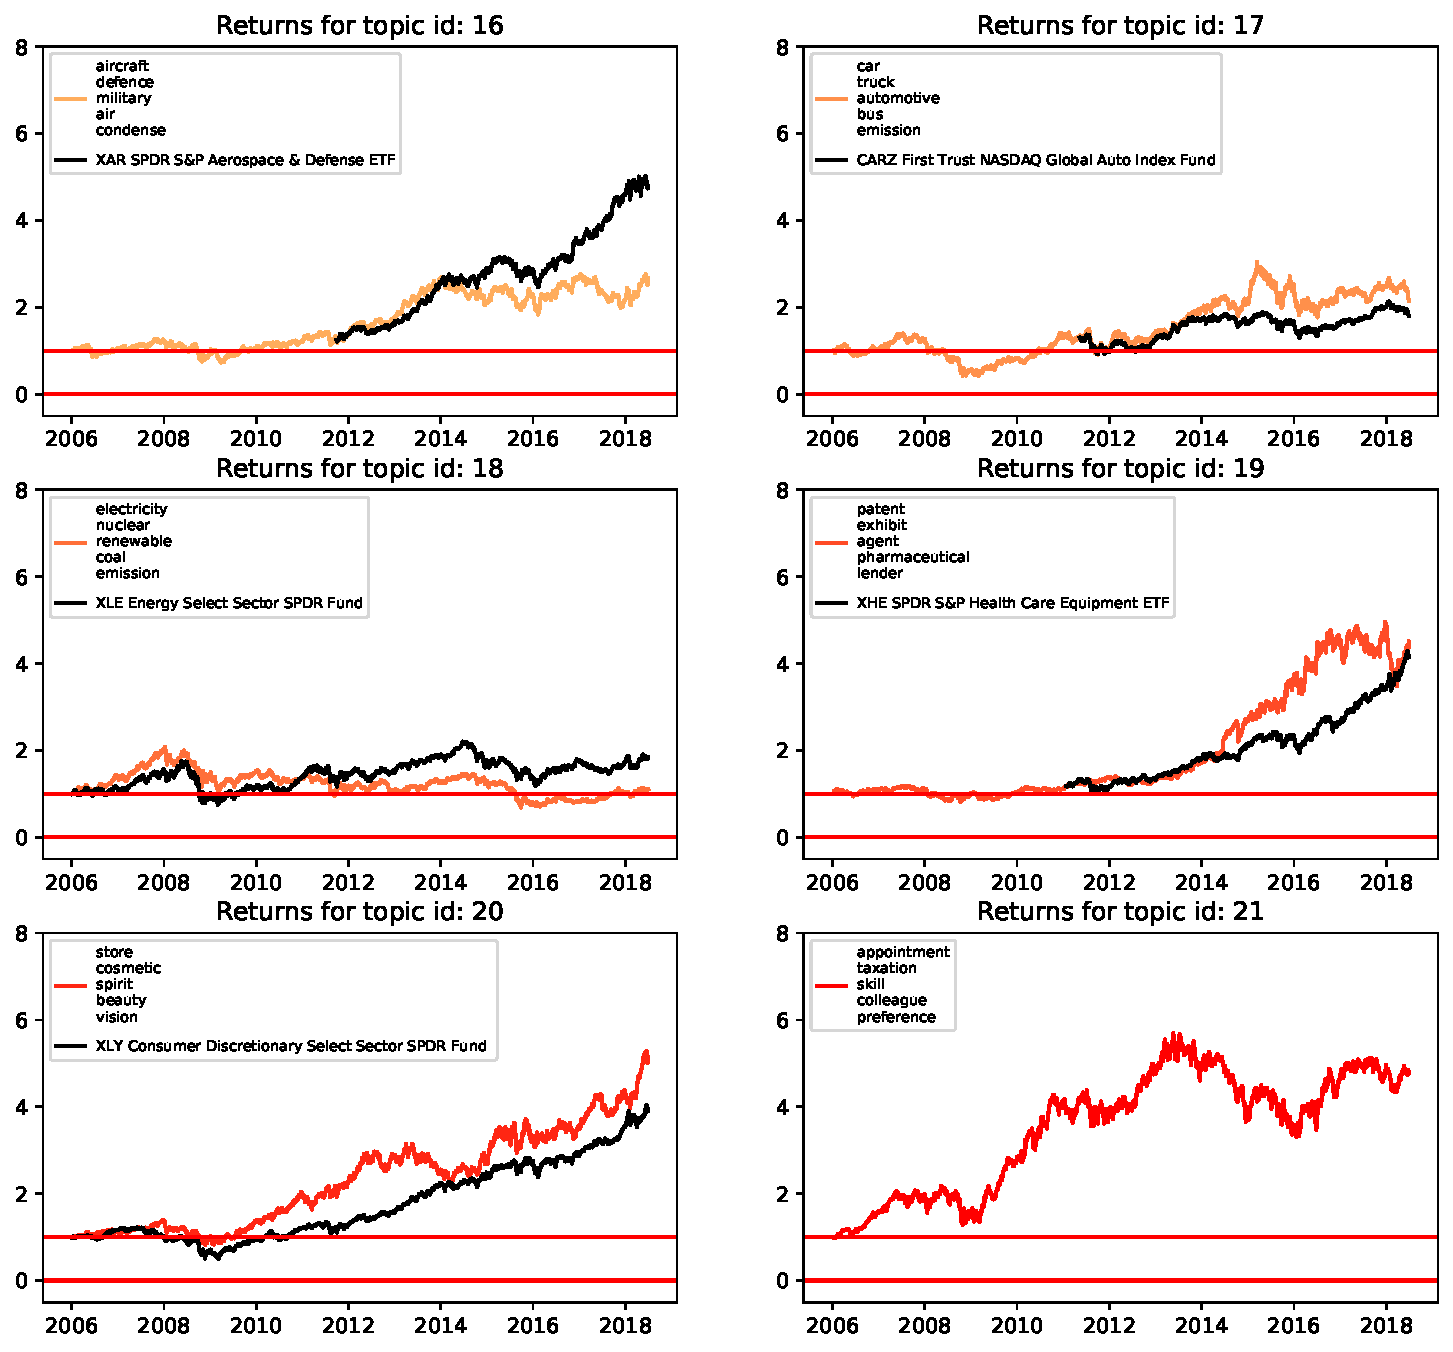
\includegraphics[width=1\linewidth]{images/returns_per_topic_page_2.pdf}
\end{center}
%\section{Appendix section 1}
%Appendix one text goes here.

% you can choose not to have a title for an appendix
% if you want by leaving the argument blank
%\section{}
%Appendix without title


% use section* for acknowledgment
%\section*{Acknowledgment}
%The authors would like to thank...  

\end{document}